\documentclass[a4paper]{oblivoir}
\author{Moon Il-chul \\ \href{mailto:icmoon@kaist.ac.kr}{icmoon@kaist.ac.kr} 
   \and Ryu Jae-hyeon
 \\ \href{mailto:ljh4773@kaist.ac.kr}{ljh4773@kaist.ac.kr} }
\setcounter{chapter}{10}
\title{Chapter 10. 샘플링 기반 추론}
\usepackage{indentfirst}
\usepackage{graphicx}
\graphicspath{ {Figure/} }
\usepackage{hyperref}
\usepackage{amsmath}
\usepackage{amssymb}
\usepackage{amsfonts}
\usepackage{dsfont}
\usepackage[]{algorithm2e}
\usepackage{chngcntr}
\counterwithin{figure}{chapter}
\setcounter{tocdepth}{2}
\setcounter{secnumdepth}{3}
\hypersetup{pdfborder={0 0 0}}
\renewcommand{\thefigure}{\thechapter-\arabic{figure}}
\renewcommand{\theequation}{\thechapter.\arabic{equation}}
\newlength\myindent
\setlength\myindent{5em}

\begin{document}
\maketitle
\tableofcontents

%\chapter{}
%-----------------------------------------------------------------
\section{기초적인 샘플링 기반 추론}
%-----------------------------------------------------------------

%-----------------------------------------------------------------
\subsection{전향 샘플링}
%-----------------------------------------------------------------

% 슬라이드 1, 2, 3
샘플링 기반 추론(Sampling Based Inference)은 수많은 경우를 추출하는 샘플링 기법을 적용해서 그래프 모델의 확률값을 구하는 추론 방법의 하나이다. Chapter 8과 chapter 9에서는 EM 알고리즘을 사용해서 파라미터가 주어지지 않은 그래프 모델의 확률값을 구하였다. 그러나 EM 알고리즘 외에 샘플링을 통해서도 확률값을 구할 수 있으며 복잡한 그래프 모델에서는 샘플링 기반 추론을 적용하는 것이 효율적인 방법이다. 샘플링의 기초적인 방법으로는 전향 샘플링, 기각 샘플링, 중요 샘플링 등의 알고리즘이 있다. 그리고 마르코프 연쇄를 적용한 메트로폴리스-헤이스팅스 알고리즘과 텍스트마이닝 등에 사용하는 깁스 샘플링과 잠재 디리클레 할당이 있으며 이것들이 우리가 여기서 다루는 내용이다. \\

%슬라이드 4
샘플링 기반 추론에서 가장 직관적인 방법으로 전향 샘플링(Forward Sampling)이 있다. 전향 샘플링에서는 베이지안 네트워크에서 제공되는 정보에 따라서 수많은 샘플을 생성하고 그것들을 바탕으로 확률을 추론한다. 이 방법은 사이클이 없는, 그에 따라서 전체 노드를 위상적 순서로 나열할 수 있는 그래프 모델에 적용할 수 있다. 여기서 위상적 순서란 그래프의 노드를 위상적 순서로 나열했을 때 모든 아크가 앞에 있는 노드에서 나와서 뒤에 있는 노드로 들어간다는 것을 의미한다. 샘플링은 맨 앞에 있는 노드부터 차례대로 이루어진다. 이 과정에서 초기 확률과 조건부 확률을 반영하여 노드의 값을 처음부터 끝까지 차례대로 생성하면서 하나의 샘플을 구성하게 된다. 이러한 과정을 계속 반복하면서 수많은 개수의 샘플을 생성한다. \\

샘플링을 위해서는 초기 확률과 조건부 확률을 프로그래밍으로 구현할 수 있어야 한다. 예를 들어, 0.3의 확률로 true가 되고 0.7의 확률로 false가 되는 확률 변수를 생성해야 한다고 하자. 이를 위해서 앞면이 나올 확률이 0.3, 뒷면이 나올 확률이 0.7인 동전을 던지는 것을 생각할 수 있다. 이 동전을 던져서 앞이 나오면 true라는 샘플을, 뒤가 나오면 false라는 샘플을 생성하는 것이다. 일반적인 프로그래밍 언어에는 난수를 생성하는 명령어가 있으며 우리는 0부터 100 사이의 수를 하나 생성하여 30 이하면 true, 30 초과면 false를 선택하는 식으로 확률 변수를 구현할 수 있다. 그리고 다항 분포나 연속 확률 분포와 같은 보다 복잡한 형태의 확률 분포 또한 난수 기능을 잘 활용한다면 프로그래밍으로 얼마든지 구현할 수 있다. \\

\begin{figure}[ht] \centering 
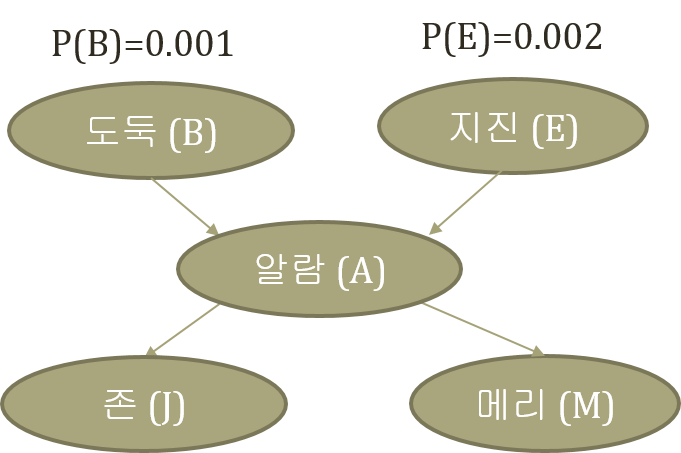
\includegraphics[scale=0.6]{fig10_1.png} 
\caption{베이지안 네트워크 예시}
\label{fig:10-1}
\end{figure} 

\begin{figure}[ht] \centering 
\parbox[t]{3cm}
{
\begin{tabular}{|c|c|c|}
  \hline
  도둑($B$) & 지진($E$) & $P(A|B,E)$ \\
  \hline
  true & true & 0.95 \\
  \hline
  true & false & 0.94 \\
  \hline
  false & true & 0.29 \\
  \hline
  false & false & 0.001 \\
  \hline
\end{tabular}
} \hspace{3cm}
\parbox[t]{5cm}
{
\begin{tabular}{|c|c|c|}
  \hline
  알람($A$) & $P(J|A)$ & $P(M|A)$ \\
  \hline
  true & 0.90 & 0.70 \\
  \hline
  false & 0.05 & 0.01 \\
  \hline
\end{tabular}
}
\caption{조건부 확률 표}
\label{fig:10-1-1}
\end{figure} 

Chapter 7에서 사용한 예시를 다시 활용해서 전향 샘플링이 무엇인지를 알아보도록 하겠다. 이 베이지안 네트워크는 위상적으로 $B$와 $E$가 앞에 있으며 $A$가 그 다음, 그리고 마지막에 $M$과 $J$가 있다. 이는 도둑이 들거나 지진이 발생하면 알람이 울릴 수 있으며, 알람이 울리면 존이나 메리가 나에게 전화를 한다는 현실적인 사건의 순서를 반영한 것이다. 이 그래프 모델에서 샘플링을 하기 위해서는 먼저 $P(B)=0.001$, $P(E)=0.002$를 반영해서 $B$와 $E$를 생성해야 한다. 이것은 $B$를 생성할 때 앞면이 나올 확률이 $0.001$, 뒷면이 나올 확률이 $0.999$인 동전을 던져서 확률을 생성해야 한다는 것을 뜻한다. 마찬가지로 $E$를 생성할 때는 앞면이 나올 확률이 $0.002$, 뒷면이 나올 확률이 $0.998$인 동전을 던져야 한다. 여기서는 $B$와 $E$가 모두 false가 나왔다고 하자. 다음으로 $A$를 생성해야 하며, $B$와 $E$가 모두 false이므로 알람이 울릴 확률은 $0.001$, 울리지 않을 확률은 $0.999$가 된다. 따라서 $A$를 생성할 때는 앞면이 나올 확률이 $0.001$, 뒷면이 나올 확률이 $0.999$인 동전을 던져야 한다. 여기서는 $A$가 true가 나왔다고 하자. 물론 확률은 $0.001$에 불과하지만 있을 수 없는 경우는 아니다. 샘플링을 수만 번, 수십만 번을 한다면 확률적으로 수십 번, 수백 번 나올 수 있는 것이다. 마지막에는 $J$와 $M$을 생성해야 한다. 알람이 울렸을 때 존이 전화를 할 확률이 $0.90$, 메리가 전화를 할 확률이 $0.70$이다. 따라서 $J$를 생성하기 위해서는 앞면이 나올 확률이 $0.90$, 뒷면이 나올 확률이 $0.10$인 동전을 던져야 한다. 그리고 $M$을 생성하기 위해서는 앞면이 나올 확률이 $0.70$, 뒷면이 나올 확률이 $0.30$인 동전을 던져야 한다. 여기서는 $J$가 true, $M$이 false가 나왔다고 하자. 이것으로 한 번의 샘플링이 끝났으며 ($B$, $E$, $A$, $M$, $J$)에 대한 하나의 샘플 (false,false,true,true,false)을 생성한 것이 된다. 우리는 샘플링을 위해서 이러한 작업을 수천 번, 수만 번, 심지어는 수십만 번이나 수백만 번을 반복해서 샘플링 횟수만큼의 샘플을 생성할 수 있다. 그리고 샘플링 과정에서의 작업 순서 결정 및 확률 계산은 베이지안 네트워크에서 주어진 위상적 구조와 사전 확률을 사용해서 이루어진다. \\

샘플링으로 확률을 계산하기 위해서는 앞에서 생성한 샘플을 하나씩 확인해서 조건에 맞는 샘플이 몇 개나 있는지를 세야 한다. 예를 들어, 존은 전화를 하지 않았지만 메리는 전화를 할 확률, 다시 말해 $J$가 false, $M$이 true일 확률을 계산해야 하는 상황이다. 여기서는 우선 이러한 경우에 해당되는 샘플이 몇 개나 있는지를 센다. 그러고 나서 $J$가 false, $M$이 true인 샘플의 개수를 전체 샘플의 개수로 나누어서 확률값을 계산하는 것이다. 조건부 확률을 구하기 위해서는 아까보다 조금 더 복잡하다. 조건부 확률을 구하기 위해서는 두 가지 사건에 대해서 각 샘플이 몇 개나 있는지를 확인해야 한다. 예를 들어, 메리가 나에게 전화를 했을 때 지진이 발생했을 확률, 다시 말해 $M$이 true일 때 $E$가 true가 되는 조건부 확률을 구하기 위해서는 먼저 조건에 해당하는 $M$이 true인 샘플이 몇 개나 되는지를 확인한다. 그러고 나서 $M$이 true이면서 $E$가 true인 샘플이 몇 개나 되는지를 세고 이것을 $M$이 true인 샘플의 개수로 나누어서 조건부 확률을 구한다. 이러한 과정은 $P(A|B)$가 $P(A,B)$에 $P(B)$를 나눈 것과 같다는 조건부 확률의 정의를 그대로 활용한 것이다. \\    

전향 샘플링은 무작위로 값을 생성하는 작업을 계속해서 반복한다. 이것을 직관적으로 이해하기는 그리 어렵지 않으며 프로그래밍으로 구현하는 것 또한 쉽고 간단하다. 그러나 전향 샘플링으로 구한 확률값을 올바른 값으로 확신하기 위해서는 수없이 많은 횟수의 반복이 이루어져야 한다. 그러나 베이지안 네트워크의 규모가 커지면 위상적 순서에 따라서 값을 하나하나 생성하는 데에는 오랜 시간이 걸린다. 거기에 더해 초기 확률이나 조건부 확률값이 극히 작은 사건에 관한 확률값을 구할 때에는 대부분의 샘플이 필요 없게 된다는 문제가 있다. 예를 들어, 도둑이 들었을 때 메리가 전화를 할 확률을 구한다고 하겠다. 전향 샘플링으로 10,000개의 샘플을 생성했다고 하면 초기 확률에 근거해서 보았을 때 도둑이 든 사건을 반영한 샘플은 100개 안팎에 불과하며 나머지 9,900개는 계산에 필요하지 않을 것이다. 이것은 시간에 있어서도, 샘플을 보관하는 메모리 공간에 있어서도 큰 낭비가 된다.   \\

%슬라이드 5
\begin{figure}[ht] \centering 
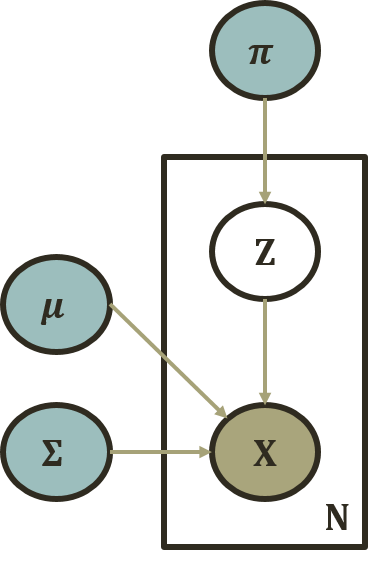
\includegraphics[scale=0.45]{fig10_2.png} 
\caption{가우시안 혼합 모델}
\label{fig:10-2}
\end{figure} 

Chapter 8에서의 가우시안 혼합 모델을 전향 샘플링으로 구현해보자. 가우시안 혼합 모델의 파라미터에는 다항 분포의 $\pi$와 다변수 가우스 분포의 $\mu, \Sigma$가 있다. 그리고 주어진 확률 변수의 위상적 순서는 $z$, 그리고 $X$의 순서이므로 샘플링은 $z \to X$ 순서로 이루어진다. 여기서는 $\pi$ 파라미터를 가지는 다항 분포에서 $z$를 먼저 샘플링한다. 그리고 샘플링한 $z$의 값에 대응하는 $\mu, \Sigma$ 파라미터를 가지는 다변수 가우스 분포에서 $X$를 샘플링한다. \\

\begin{figure}[ht] \centering 
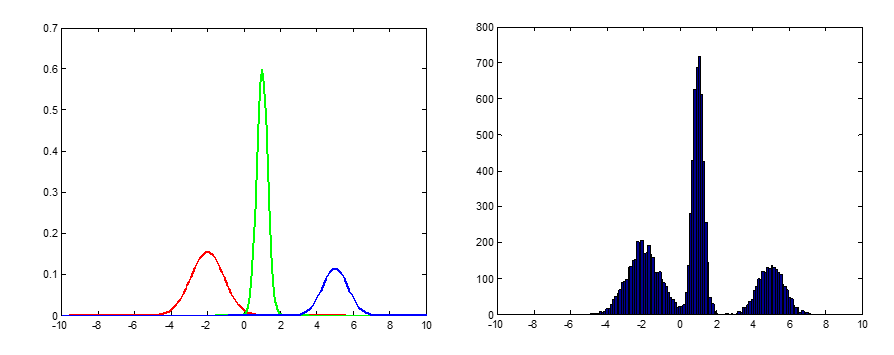
\includegraphics[scale=0.45]{fig10_3.png} 
\caption{가우시안 혼합 모델에서의 전향 샘플링 결과}
\label{fig:10-3}
\end{figure}  

그림 \ref{fig:10-3}의 오른쪽 그래프는 샘플링한 $X$값들을 그래프 위에 나타낸 것이다. 이것의 형태는 왼쪽의 가우시안 혼합 모델의 확률 밀도  함수와 거의 일치한다. 이처럼 확률 밀도 함수를 알 수 없는 그래프 모델에 대해서도 충분한 횟수의 샘플링을 한다면 확률 밀도 함수의 개형을 어렵지 않게 그릴 수 있다. 그러나 앞에서 설명한 단점들 때문에 전향 샘플링을 사용하는 것은 대체로 적절하지 않으며, 다른 샘플링 방법이 필요하다. 

%-----------------------------------------------------------------
\subsection{기각 샘플링}
%-----------------------------------------------------------------

%슬라이드 6
앞서 설명한 전방 샘플링의 약점을 다소나마 보완한 샘플링으로 기각 샘플링이 있다. 기각 샘플링(Rejection Sampling)은 샘플링을 진행하면서 구하려 하는 확률의 조건과 관련된 샘플만을 취하고 그 외의 샘플은 버리는 방법이다. 이것은 전방 샘플링처럼 샘플링을 여러 번 해서 확률값을 구하는 방법이다. 그러나 앞서의 전방 샘플링에서 확률의 조건을 생각하지 않고 샘플을 생성하는 것과는 달리 기각 샘플링에서는 샘플링 중간중간에 확률의 조건에 맞지 않는 샘플은 버리고 맞는 샘플만을 모아서 확률값을 계산한다. \\

\begin{figure}[ht] \centering 
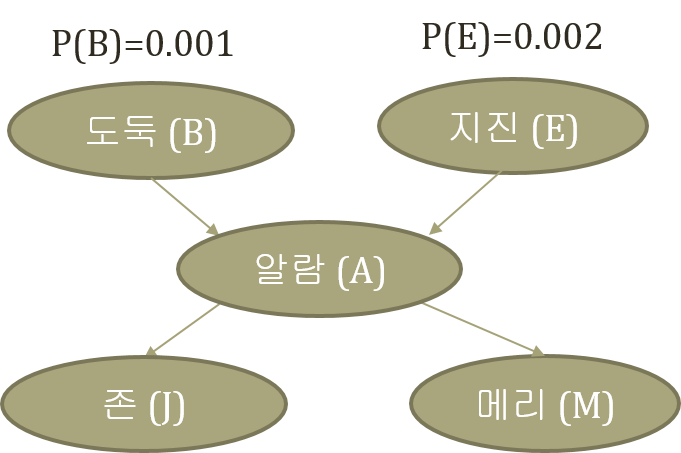
\includegraphics[scale=0.6]{fig10_1.png} 
\caption{베이지안 네트워크 예시}
\label{fig:10-1-2}
\end{figure} 

\begin{figure}[ht] \centering 
\parbox[t]{3cm}
{
\begin{tabular}{|c|c|c|}
  \hline
  도둑($B$) & 지진($E$) & $P(A|B,E)$ \\
  \hline
  true & true & 0.95 \\
  \hline
  true & false & 0.94 \\
  \hline
  false & true & 0.29 \\
  \hline
  false & false & 0.001 \\
  \hline
\end{tabular}
} \hspace{3cm}
\parbox[t]{5cm}
{
\begin{tabular}{|c|c|c|}
  \hline
  알람($A$) & $P(J|A)$ & $P(M|A)$ \\
  \hline
  true & 0.90 & 0.70 \\
  \hline
  false & 0.05 & 0.01 \\
  \hline
\end{tabular}
}
\caption{조건부 확률 표}
\label{fig:10-1-1-2}
\end{figure} 

전방 샘플링에서 사용했던 베이지안 네트워크 예시를 다시 불러와서 확률값을 계산해보자. 알람이 울리지 않았으나 메리가 나에게 전화를 했을 때 지진이 발생했을 확률, 다시 말해 $A$가 false, $M$이 true라는 조건이 주어졌을 때 $E$가 true일 조건부 확률을 구한다고 하자. 여기서도 개별 샘플의 생성은 $B$와 $E$, $A$, 그리고 $J$와 $M$의 순서로 이루어진다. 먼저 $B$와 $E$를 생성하자. 여기서는 각각 false와 true가 나왔다고 하겠다. 조건부 확률의 조건은 $A$, $M$과 관련이 있으므로 그대로 넘어가도 좋다. 다음으로 $A$를 생성하자. $B$와 $E$가 각각 false와 true이므로 $A$가 true일 확률 $0.29$, false일 확률 $0.71$에 맞춰서 $A$를 생성해야 한다. 여기서 $A$가 false가 나왔다면 조건부 확률의 조건과 일치하므로 다음으로 넘어가면 된다. 그러나 $A$가 true가 나왔다면 조건부 확률의 조건과 맞지 않으므로 이 샘플을 기각하고 맨 처음으로 돌아가서 새로운 샘플을 생성해야 한다. 같은 식으로 $J$와 $M$에 대해서도 $J$는 조건과 관련이 없으므로 true, false 중에서 어떤 값이 나오더라도 샘플을 기각할 수 없지만 $M$은 $M$이 true여야 한다는 조건이 있으므로 false가 나온다면 그 샘플은 기각하고 처음부터 새로운 샘플을 만들어야 한다. \\

이렇게 조건부 확률의 조건과 일치하지 않는 샘플을 중간에서 모두 기각해 가면서 샘플링을 한다면 결과로 나오는 샘플들은 모두 조건을 만족하는 샘플이 된다. 우리는 여기서 조건부 확률의 사건에 해당되는 샘플만을 세어서 그 개수가 얼마나 되는지를 확인할 수 있다. 그리고 이를 전체 샘플의 개수로 나누어서 원하는 조건부 확률값을 구할 수 있다. \\

%슬라이드 7
\begin{figure}[ht] \centering 
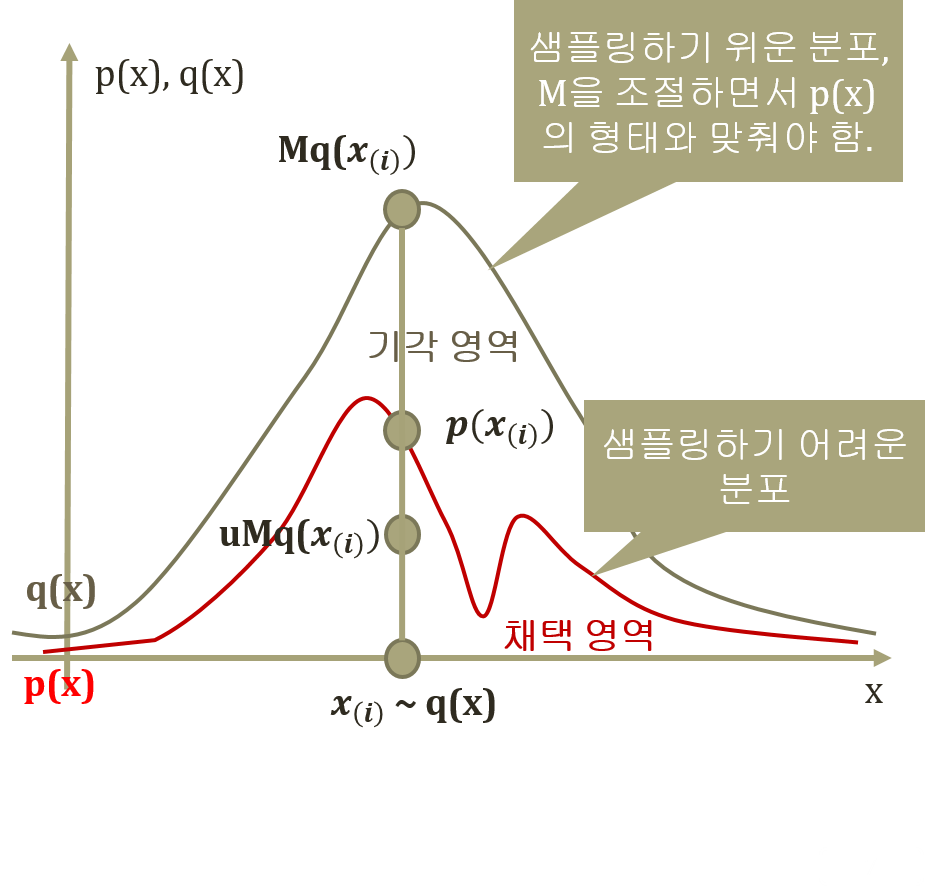
\includegraphics[scale=0.45]{fig10_4.png} 
\caption{연속 확률 분포에서의 기각 샘플링}
\label{fig:10-4}
\end{figure}  

앞에서의 이산 확률 분포 외에 연속 확률 분포 또한 기각 샘플링을 통해서 생성할 수 있다. 그림 \ref{fig:10-4}에서 확률 밀도 함수가 빨간색 그래프 $p(x)$인 확률 변수에 대해서 어떻게 샘플링을 할지 확인해 보겠다. 이 경우 각 $x$에 대한 확률 밀도 함수의 값 자체를 구할 수는 있지만 분포 함수의 형태가 익숙한 형태가 아니기 때문에 샘플링하기는 쉽지 않다. 여기서는 먼저 우리가 잘 알고 있는 정규분포 함수 $q(x)$를 정한다. 그리고 모든 $x$에 대해서 $p(x)$ 위에 있도록 $q(x)$에 양의 상수 $M$을 곱해서 $Mq(x)$를 구한다. 여기서 사실은 $Mq(x)$가 모든 $x$에서 $p(x)$보다 크려면 처음부터 정규분포의 평균과 표준편차의 값을 잘 정의해 주어야 한다. \\

기각 샘플링의 원리는 분포 함수의 값을 구하기는 쉽지만 샘플링하기에는 쉽지 않은 확률 변수에 대해서 샘플의 생성 과정을 두 부분으로 나누는 것에 있다. 기각 샘플링을 위해서 먼저 정규분포 함수가 $q(x)$인, 평균과 표준편차를 사전에 정한 정규분포로부터 샘플 $x_{(i)}$를 생성한다. 그러고 나서 [0,1] 범위에서 균등한 분포를 나타내는 연속균등분포(Continuous Uniform Distribution)로부터 샘플 $u_{(i)}$를 생성한다. 여기서 $p(x_{(i)})/Mq(x_{(i)})$가 $u_{(i)}$보다 크면 샘플 $x_{(i)}$를 취하고 $u_{(i)}$보다 작거나 같으면 샘플 $x_{(i)}$를 기각한다. 이러한 작업을 원하는 개수만큼의 샘플이 모일 때까지 반복하는 것이 연속 확률 분포에 대한 기각 샘플링이 된다. \\  

전향 샘플링과 비교하면 기각 샘플링에서는 쓸모 없는 샘플이 생성되는 것을 막을 수 있다는 장점이 있다. 그러나 기각 샘플링에서는 모든 $x$에서 $p(x)$보다 큰 $Mq(x)$가 되는 양의 상수 $M$과 샘플링하기 쉬운 $q(x)$를 찾아야 하지만 이것은 쉽지 않은 작업이다. 우선, 다루기 용이하면서도 샘플링을 원하는 확률 분포인 $p(x)$와 유사한 형태의 $q(x)$를 찾기가 쉽지 않다. 그리고 적절한 $q(x)$를 찾았다고 하더라도 양의 상수 $M$을 너무 작게 잡으면 몇몇 $x$에서 $Mq(x)$가 $p(x)$보다 작게 되어 올바른 기각 샘플링이 되지 않을 수 있다. 반면에 양의 상수 $M$을 너무 큰 수로 잡으면 기각되는 샘플이 올바른 샘플에 비해서 훨씬 많이 생성되면서 샘플링의 반복 횟수가 늘어나 시간이 오래 걸릴 수 있다. 연속 확률 분포 외에 $M$과 $q(x)$를 생각할 필요가 없는 이산 확률 변수에서의 전향 샘플링에 대해서도 샘플이 자주 기각되면서 알고리즘의 작동 시간이 늘어나는 것이 문제였는데 이러한 문제가 다시 한 번 발생하는 것이다.  \\

%슬라이드 8
그러나 설령 앞에서와 같은 문제가 있다고 하더라도 기각 샘플링으로 chapter 8에서의 혼합 모델을 샘플링할 수 있다. 실제로 가우시안 혼합 모델에 기각 샘플링 과정을 진행하면서 그것을 알아보도록 하겠다.  

\begin{figure}[ht] \centering 
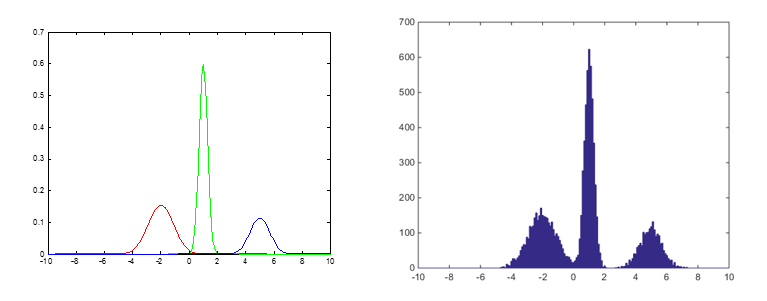
\includegraphics[scale=0.8]{fig10_5.png} 
\caption{가우시안 혼합 모델과 기각 샘플링 결과 1}
\label{fig:10-5}
\end{figure}  

우리는 여러 개의 정규분포를 결합한 혼합 모델을 샘플링하려고 한다. 여기서 혼합 모델의 $p(x)$는 평균이 $-2$, 표준편차가 $0.9$인 정규분포 함수, 평균이 $1$, 표준편차가 $0.3$인 정규분포 함수, 그리고 평균이 $5$, 표준편차가 $0.8$인 정규분포 함수에 $0.35$, $0.45$, 그리고 $0.2$를 각각 곱한 뒤에 그것들을 모두 더해서 만든 확률 밀도 함수이다. 우리는 평균이 $-2$, 표준편차가 $1$인 정규분포 함수, 평균이 $1$, 표준편차가 $1$인 정규분포 함수, 그리고 평균이 $5$, 표준편차가 $1$인 정규분포 함수를 $1/3$씩 결합해서 만든 확률 밀도 함수 $q(x)$를 사용해서 기각 샘플링을 진행하였다. 이들 함수에는 세 개의 봉우리를 가지고 있으며, 이들 세 봉우리의 $x$좌표 위치가 각각 $-1$, $2$, $5$로 일치하는 등 형태에 있어서 상당한 유사점을 가진 것으로 보인다. 그림 \ref{fig:10-5}은 기각 샘플링의 결과를 나타낸다. 샘플링 결과를 $p(x)$의 형태와 비교한다면 거의 비슷한 형태를 나타내고 있으며, 따라서 샘플링이 잘 되었다고 생각할 수 있다. 이러한 샘플링 결과는 무엇보다도 $p(x)$와 형태가 거의 비슷하도록 $q(x)$를 정했기 때문에 가능한 것이다. 기각 샘플링 과정에서 $q(x)$에 적당한 크기의 상수인 $M$을 곱해서 $p(x)$보다 더 크면서도 $p(x)$와 비슷한 형태를 가진 $Mq(x)$를 구성하면서 정교한 기각 샘플링이 되었다. \\

\begin{figure}[ht] \centering 
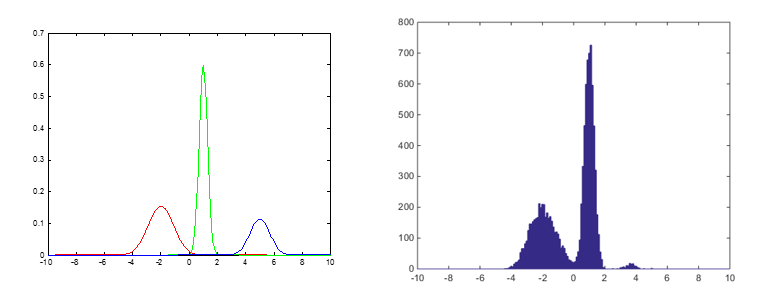
\includegraphics[scale=0.8]{fig10_6.png} 
\caption{가우시안 혼합 모델과 기각 샘플링 결과 2}
\label{fig:10-6}
\end{figure}  

한편, 이번에는 평균이 $0$, 표준편차가 $1$인 정규분포 함수를 $q(x)$로 정의하고 기각 샘플링 과정을 진행하도록 하겠다. 첫 번째의 $q(x)$와 비교했을 때 이번 $q(x)$는 $p(x)$와 형태에 있어서 비교적 많은 차이가 나타난다. 그리고 이것은 샘플링의 결과에 크게 영향을 미칠 것이다. 그림 \ref{fig:10-6}의 샘플링 결과를 보면 $p(x)$와 비교했을 때 첫 번째와 두 번째 봉우리는 잘 나타내었으나 세 번째 봉우리가 거의 나타나지 않았음을 확인할 수 있다. 이는 $M$을 충분히 크게 잡지 못했기 때문에 세 번째 봉우리가 자리할 위치에서는 $p(x)$가 $Mq(x)$보다 더 크기 때문에 나타나는 문제이다. 이러한 문제를 극복하기 위해서는 $M$을 더더욱 크게 잡아야 한다. 그러나 앞에서도 설명했다시피 $M$이 커지면 샘플을 기각할 확률 역시 높아지기 때문에 전체 샘플링 시간이 늘어난다는 문제점을 가지고 있다. 그 때문에 크고 복잡한 형태의 베이지안 네트워크 추론에 기각 샘플링은 그렇게 적절하지 않으며 이를 극복할 수 있는 대안으로서의 샘플링 방법 또한 존재한다. 

%-----------------------------------------------------------------
\subsection{중요 샘플링}
%-----------------------------------------------------------------

%슬라이드 9
앞서의 전향 샘플링이나 기각 샘플링에서는 버려지거나 기각되는 샘플이 많아지면서 전체 샘플링 시간이 길어진다는 것이 문제였다. 이를 보완할 수 있는 방법의 하나로 중요 샘플링이 있다. 중요 샘플링(Importance Sampling)은 원하는 확률값이나 기댓값을 구하는 것을 직접적인 목표로 샘플링을 하는 샘플링을 말한다. 전향 샘플링이나 기각 샘플링에서는 샘플링 결과를 바탕으로 히스토그램을 그려서 확률 모델의 확률 밀도 함수를 직접 나타내었다. 그러나 이제는 확률 밀도 함수를 직접 구할 필요 없이 확률 밀도 함수의 기댓값이나 원하는 확률값만을 구하면서 계산량을 크게 줄일 수 있다. \\

먼저 중요 샘플링으로 확률 모델의 기댓값을 구하는 과정을 생각해보자. 여기서는 확률 모델에 관련된 확률 변수 $z$와 그것의 확률 분포 $p(z)$가 있고 임의의 함수인 $f(z)$가 있다고 하겠다. 이 때 $f(z)$의 기댓값을 다음과 같이 나타낼 수 있다.
\begin{equation}
E[f(z)] = \int_{z} f(z)p(z)dz
\label{eq:10-1}
\end{equation} 
여기서 우리는 $p(z)$를 정확히 모르기 때문에 더 이상 식을 전개할 수 없다. 여기서 더 나아가기 위해서는 먼저 새로운 함수인 $q(z)$를 도입해야 한다. 그러면 다음과 같이 식을 전개할 수 있다.
\begin{eqnarray}
E[f(z)] & = & \int_{z} f(z)p(z)dz \nonumber \\
& = & \int_{z} f(z) \frac{p(z)}{q(z)} q(z) dz \nonumber \\
& \cong & \frac{1}{L} \sum_{l=1}^{L} \frac{p(z^{l})}{q(z^{l})}f(z^{l}) \label{eq:10-2}
\end{eqnarray} 
여기서는 수식 (\ref{eq:10-2})의 두 번째 줄의 식을 $q(z)dz$ 부분을 $1/L$로, 적분 기호를 시그마로 전환해서 세 번째 줄의 식으로 근사하였다. 이는 $z$값이 하나 주어졌을 때 정확한 $p(z)$의 값을 구하는 것은 가능하지만 무한대로 많은 $z$에 대한 확률 계산이 되는 적분식을 더 이상 전개할 수 없기 때문이다. 여기서는 총 $L$개의 $z^{l}$ 샘플을 사용했으며 이들은 샘플링 분포로부터 $L$번 샘플링을 진행한 결과이다. 그리고 여기에는 중요 가중치(Importance Weight)라고 부르는 중요한 의미를 가지는 가중치가 있다. 
\begin{equation}
r^{l} = \frac{p(z^{l})}{q(z^{l})}
\label{eq:10-2-1} 
\end{equation} 
여기서 $p(z^{l})$와 $q(z^{l})$이 정규화되지는 않았지만 $z_{p}$와 $z_{q}$라는 정규화 상수를 도입해서 $p$와 $q$를 확률 분포 함수인 $\tilde{p}$와 $\tilde{q}$로 바꿔서 $E[f(z)]$에 관한 원래의 식을 다음과 같이 바꿔서 표현할 수 있다. 
\begin{eqnarray}
E[f(z)] & \cong & \frac{1}{L} \sum_{l=1}^{L} \frac{p(z^{l})}{q(z^{l})}f(z^{l}) \nonumber \\
& = &  \frac{1}{L} \frac{z_{q}}{z_{p}} \sum_{l=1}^{L} \frac{\tilde{p}(z^{l})}{\tilde{q}(z^{l})}f(z^{l}) \label{eq:10-2-2}
\end{eqnarray} 

다음으로 중요 샘플링으로 잠재 변수 $z$가 1보다 크거나 같을 확률을 계산해 보겠다. 이를 위해서는 $z$가 1, 2 또는 그 이상인 경우의 $p(z)$의 값은 모두 더하고 그 외에 $z$가 0이거나 음수인 경우의 $p(z)$의 값은 생각하지 않으면 된다. 이러한 사실을 수식으로 나타내면 다음과 같이 나온다.
\begin{equation}
P(z \geq 1) = \int_{z \geq 1} p(z)dz
\label{eq:10-2-3}
\end{equation} 
그러나 이것 또한 직접 구하기는 쉽지 않기 때문에 여기서부터는 샘플링을 통해서 값을 구해야 한다. 샘플링을 위해서는 먼저 $q(z)$라는 샘플링 분포를 정해서 원래의 적분식을 다음과 같은 식으로 바꿔야 한다. 
\begin{equation}
P(z \geq 1) = \int_{z \geq 1} \frac{p(z)}{q(z)} q(z) dz
\label{eq:10-2-4}
\end{equation} 
그리고 샘플링 결과인 $L$개의 $z^{l}$ 데이터를 활용해서 적분식을 근사하면 이것을 다음과 같이 샘플링의 결과값으로 구성된 항들을 모두 합한 식으로 나타낼 수 있다.
\begin{equation}
P(z \geq 1) = \frac{1}{L} \sum_{l=1}^{L} \frac{p(z^{l})}{q(z^{l})} 1_{z^{l} \geq 1}
\label{eq:10-2-5}
\end{equation} 
여기서 $1_{z^{l} \geq 1}$은 $z^{l}$이 $1$보다 크거나 같으면 $1$의 값을, 그 외에는 $0$의 값을 가지는 함수이다. 이것을 앞에서 $E[f(z)]$을 풀어서 쓴 식과 비교해보면 원래의 $f(z^{l})$가 $1_{z^{l} \geq 1}$로 정해진 특수한 경우에 해당함을 알 수 있다. 이런 식으로 적분을 하기 어려운 혼합 모델의 확률에 대해서도 샘플링을 적용하면 손쉽게 그 값을 구하는 것이 가능하다.   

%슬라이드 10
\begin{figure}[ht] \centering 
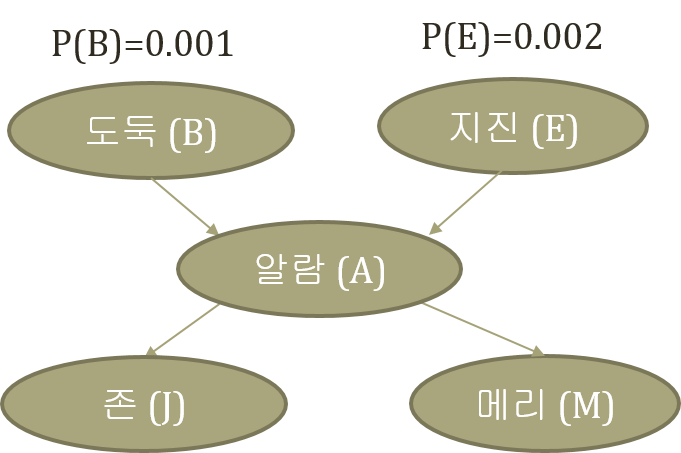
\includegraphics[scale=0.6]{fig10_1.png} 
\caption{베이지안 네트워크 예시}
\label{fig:10-1-3}
\end{figure} 

\begin{figure}[ht] \centering 
\parbox[t]{3cm}
{
\begin{tabular}{|c|c|c|}
  \hline
  도둑($B$) & 지진($E$) & $P(A|B,E)$ \\
  \hline
  true & true & 0.95 \\
  \hline
  true & false & 0.94 \\
  \hline
  false & true & 0.29 \\
  \hline
  false & false & 0.001 \\
  \hline
\end{tabular}
} \hspace{3cm}
\parbox[t]{5cm}
{
\begin{tabular}{|c|c|c|}
  \hline
  알람($A$) & $P(J|A)$ & $P(M|A)$ \\
  \hline
  true & 0.90 & 0.70 \\
  \hline
  false & 0.05 & 0.01 \\
  \hline
\end{tabular}
}
\caption{조건부 확률 표}
\label{fig:10-1-1-3}
\end{figure} 

이제는 전향 샘플링과 기각 샘플링을 설명하는데 사용했던 베이지안 네트워크를 다시 가져와서 이야기를 진행해 보겠다. 이러한 확률 모형에서의 확률값을 중요 샘플링으로 어떻게 구할 수 있을까. 여기서도 알람은 울리지 않았으나 메리가 나에게 전화를 했다는 상황에서 지진이 발생했을 확률을 구하려 한다. 이것은 다시 말해 $A$가 false, $M$이 true라는 조건이 주어졌을 때 $E$가 true일 조건부 확률을 구한다는 것이다. \\

하나의 샘플을 생성하는 샘플링 과정 자체는 전향 샘플링이나 기각 샘플링과 같은 순서로 진행하나 여기에는 약간의 차이가 있다. 중요 샘플링 과정에서도 변수가 잠재 변수인 경우에는 초기 확률 및 조건부 확률을 바탕으로 무작위로 샘플링을 진행해서 변수들에 값을 할당한다. 그러나 변수가 관찰 변수인 경우에는 관찰된 그대로 값을 할당한다. 예시에서는 다음과 같은 순서로 샘플링을 진행할 수 있다. 먼저 $B$와 $E$는 잠재 변수이므로 초기 확률을 바탕으로 무작위로 값을 생성한다. 여기서는 각각 false, false가 할당되었다고 하겠다. 다음으로는 $A$가 있으나 이것은 관찰 변수이므로 조건에서 주어진 관찰값인 false를 할당한다. 마지막으로 $J$와 $M$에 대해서는 $J$는 잠재 변수이지만 $M$은 관찰 변수이므로 이들을 각각 다르게 취급해야 한다. 여기서는 무작위로 생성한 결과 $J$에는 true가 할당되었다고 하겠다. 한편, $M$에는 이미 주어진 값인 true를 할당해야 한다. 우리는 샘플링의 결과로 나온 샘플 하나하나가 조건부 확률의 조건을 만족한다는 것을 알 수 있다. 따라서 이러한 과정을 반복한다면 중요 샘플링에 사용하는 샘플을 계속해서 생성할 수 있다. 그러나 이렇게 생성한 샘플들을 모두 똑같이 취급할 수는 없다. 관찰 변수에 주어진 값을 그대로 할당하는 것이 샘플에 따라서 확률적으로 적절한 경우도 있지만 그렇지 않은 경우도 있기 때문이다. \\

중요 샘플링에서는 샘플을 생성한 이후나 생성하는 도중에 주어진 조건에 맞지 않는다는 이유로 샘플을 무시하거나 기각하지 않는다. 그 대신 조건에 맞도록 생성한 샘플에 가중치를 설정해서 올바른 샘플링이 되도록 한다. 이러한 가중치에는 샘플이 실제로 나오게 되는 확률값이 반영되어 있다. 생성한 샘플의 샘플링 가중치를 계산하기 위해서는 먼저 우리가 구하고자 하는 조건부 확률의 조건에 해당되는 각각의 변수가 샘플링 과정에서 할당된 값과 똑같이 나올 확률을 확인해야 한다. 여기서 가중치 외의 변수의 값은 샘플링 과정에서 할당된 값으로 고정되었다고 가정하므로 이러한 확률값들은 초기 확률 및 조건부 확률을 통해서 확인할 수 있다. 그리고 확인한 확률값들을 모두 곱해서 생성한 샘플의 샘플링 가중치로 둔다. 이런 식으로 각각의 샘플에 대해서 샘플이 실제로 생성될 확률을 가중치로 놓고 샘플끼리 차이를 둘 수 있는 것이다. \\

실제로 중요 샘플링을 구현하기 위해서는 샘플링 중간중간에 우리가 구하고자 하는 조건부 확률의 조건에 해당되는 변수가 나올 때마다 이를 샘플링 가중치에 반영하는 것이 좋다. 여기서는 샘플을 생성하기 전에 먼저 샘플링 가중치 값을 1로 놓고 시작한다. 그리고 $A$에 false를 할당할 때 원래의 가중치 값인 1에 $B$와 $E$가 각각 false일 때 $A$가 false일 조건부 확률인 0.999를 곱한 0.999를 새로운 가중치 값으로 둔다. 이어서 $M$에 true를 할당할 때 원래의 가중치 값인 0.999에 $A$가 false일 때 $M$이 true일 조건부 확률인 0.01을 곱한 0.00999를 새로운 가중치 값으로 둔다. $M$ 이후에는 더 이상 생각할 변수가 없으므로 이 샘플에 대한 샘플링 가중치는 0.00999가 된다. 이러한 과정을 샘플 생성 과정과 함께 병행하면서 샘플과 함께 샘플의 가중치를 내놓는 것이 바로 중요 샘플링의 과정이 된다. \\

이러한 중요 샘플링의 결과로 나온 샘플을 바탕으로 우리가 원하는 확률값을 구하기 위해서는 먼저 확률의 사건에 해당되는 샘플의 가중치만을 모두 더해야 한다. 그리고 이렇게 더한 값을 모든 샘플의 가중치의 합으로 나누어서 확률값을 계산해야 한다. 예를 들어, 예시에서의 조건부 확률을 구하기 위해서는 먼저 $E$가 true인 샘플만을 찾아서 그것들의 가중치를 모두 더해야 한다. 그리고 그 값으로 전체 샘플의 가중치를 모두 더한 값에 나누는 정규화 과정을 거치면 우리가 원하는 확률값을 구할 수 있다. 

%-----------------------------------------------------------------
\section{깁스 샘플링}
%-----------------------------------------------------------------

%-----------------------------------------------------------------
\subsection{마르코프 연쇄}
%-----------------------------------------------------------------

%슬라이드 11
앞서서 우리는 전향 샘플링, 기각 샘플링, 중요 샘플링을 다뤘으나 이것들은 기초적이며 이론적인 모델에 가깝다. 한편, 기계 학습에서 샘플링 기반의 추론에 쓰이는 핵심 알고리즘으로는 깁스 샘플링이 있다. 그리고 메트로폴리스-헤이팅스 알고리즘은 깁스 샘플링의 일반적인 경우이다. 현실에서 주로 사용하는 두 가지 샘플링을 알아보고 이것들이 실제로 어떻게 적용되는지를 살펴보도록 하겠다. \\

샘플링 기반 추론의 한 방법인 메트로폴리스-헤이팅스 알고리즘을 살펴보기 위해서는 먼저 EM 알고리즘을 이해하고 있어야 한다. Chapter 8, 9에서 가우시안 혼합 모델과 마르코프 은닉 마르코프 모델의 확률값을 구하기 위해서 EM 알고리즘을 사용했었다. 우리는 그 때 EM 알고리즘의 이론적 토대를 설명하기 위해서 $P(X|\theta)$에서 잠재 변수를 꺼내고 로그를 취하는 등의 변화를 주면서 $\textrm{ln} \{ \sum_{z} P(X, z|\theta) \}$로 나타내었다. EM 알고리즘은 기댓값 과정과 최대화 과정의 두 가지 과정을 번갈아가면서 행하는 알고리즘이다. 이들은 각각 $z$의 확률 분포 함수 $q(z)$를 구하는 과정과 파라미터 $\theta$의 값을 구하는 과정이 된다. 샘플링 기반 추론이 활용되는 부분은 기댓값 과정이며, 정확히는 $P(X, z|\theta)$를 샘플링 기반 추론으로 구하는 것을 말한다. 지금까지의 기댓값 과정은 어디까지나 $z$를 구성하는 최적의 분포인 $q(z)$를 찾는 것이 주 목적이였다. 그러나 이번에는 $z$를 지속적으로 샘플링하면서 $z$의 분포를 구성하고 그것을 바탕으로 최대화 과정에서 파라미터의 값을 구해야 한다. \\

샘플링 기반 추론이 일반적인 가우시안 혼합 모델에 잘 적용된다고는 할 수 없다. 그러나 여러 단계의 잠재 변수가 순차적으로 연결되어 있을 때에는 깁스 샘플링을 적용해서 확률값을 계산할 수 있다. 현실에서는 텍스트마이닝을 위한 약한 군집화 모델 등에서 깁스 샘플링을 활용한다. 그러나 깁스 샘플링을 이해하고 실제로 구현하려면 먼저 마르코프 연쇄에 대한 이해가 필요하다. 왜냐하면 지금까지의 샘플링에서는 먼저 만들어진 인스턴스와 나중에 만들어진 인스턴스 사이의 관계가 없지만 메트로폴리스-헤이팅스 알고리즘이나 깁스 샘플링에서는 먼저 만들어진 인스턴스와 나중에 만들어진 인스턴스 사이에 나름의 관계가 있기 때문이다. 따라서 이러한 인스턴스 사이의 시간적 관계를 반영할 수 있는 마르코프 연쇄를 잘 이해하고 있어야 메트로폴리스-헤이팅스 알고리즘이나 깁스 샘플링이 왜, 어떻게 작동하는지를 이해할 수 있다. \\

%슬라이드 12
\begin{figure}[ht] \centering 
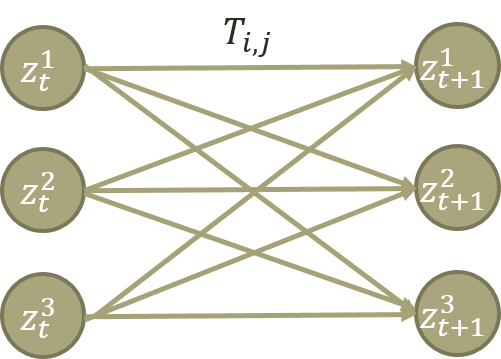
\includegraphics[scale=0.8]{fig10_8.png} 
\caption{마르코프 연쇄 예시}
\label{fig:10-8}
\end{figure}  
마르코프 연쇄(Markov Chain)는 시간에 따른 상태의 변화를 각 노드별로 나가는 아크의 확률의 합이 정확히 1이 되는 그래프로 나타낼 수 있는 이산적 형태의 확률 과정을 말한다. 여기서 확률 과정(Stochatic Process)이라는 표현을 쓴 까닭은 특정 시점에서의 상태에 대한 정보가 해당 시점에서의 정확한 관찰 결과가 아닌 이전 시점의 상태에 따른 확률값으로 나타내어지기 때문이다. 확률적인 관점에서 보면, 시간 $t$에서 확실한 관찰이 있었다면 관찰된 특정 상태일 확률은 정확히 $1$이지만 그 외의 상태일 확률은 $0$이 된다. 그러나 마르코프 연쇄에서는 특정 시점에서의 정확한 관찰 정보가 주어져 있지 않으며, 주어진 정보는 시간 $t$에서의 상태가 주어졌을 때 바로 다음 시점인 시간 $t+1$에서 될 수 있는 상태에 대한 각각의 확률값 뿐이다. \\
 
그림 \ref{fig:10-8}에서 주어진 그래프는 마르코프 연쇄의 대표적인 예시이다. 여기에는 특정 시간 $t$와 $t+1$에서의 상태가 각각 있고 시간 $t$의 상태에서 시간 $t+1$의 상태로 전이(Transition)가 일어난다. 그리고 시간 $t$의 상태 $i$에서 시간 $t+1$의 상태 $j$로 넘어갈 확률을  $T_{i,j}$로 두었으며 앞에서도 설명했듯이 이것이 우리에게 주어진 정보의 전부이다. 우리는 $T_{i,j}$ 값들을 모아서 다음과 같은 전이 행렬(Transition Matrix) $T$로 나타낼 수 있다. 
\begin{equation}
T = P(z_j|z_i) = \left( \begin{array}{ccc} T_{1,1} & T_{1,2} & T_{1,3} \\ T_{2,1} & T_{2,2} & T_{2,3} \\ T_{3,1} & T_{3,2} & T_{3,3} \end{array} \right) = \left( \begin{array}{ccc} 0.7 & 0.2 & 0.1 \\ 0.2 & 0.3 & 0.5 \\ 0.4 & 0.2 & 0.4 \end{array} \right) 
\label{eq:10-3}
\end{equation} 
그림 \ref{fig:10-8}의 마르코프 연쇄를 이해하기 위해서 수식 (\ref{eq:10-3})의 전이 행렬을 분석해 보자. 먼저 시간 $t$와 $t+1$에는 각각 $1$, $2$, $3$번의 세 개의 상태가 있다. 그리고 첫 번째 상태에서 상태를 유지할 확률은 $T_{1,1}$에 해당되는 $0.7$이며, 두 번째 상태로 넘어갈 확률은 $0.2$, 세 번째 상태로 넘어갈 확률은 $0.1$이 된다. 전이 행렬의 특징 중에서 가장 중요한 것은 각 행의 값을 모두 합하면 그것은 정확히 1이 되어야 한다는 것이다. 이것은 수식 (\ref{eq:10-3})의 전이 행렬에 대해서도 그대로 성립해서 첫 번째, 두 번째, 그리고 세 번째 행을 합하면 정확히 1이 된다는 것을 알 수 있다. \\

전이 행렬을 통해서 확률의 변화가 실제로 어떤 식으로 일어나는지를 생각해보자. 먼저 시간 $t$에서 첫 번째 상태일 확률을 $0.5$, 두 번째 상태일 확률을 $0.2$, 그리고 세 번째 상태일 확률을 $0.3$으로 가정하였다. 그러면 시간 $t+1$에서 각각의 상태로 나타날 확률을 앞에서의 확률과 전이 행렬을 이용해서 계산할 수 있다. 예를 들어, 시간 $t+1$에서 첫 번째 상태일 확률은 시간 $t$에서 각각의 상태일 확률인 $0.5$, $0.2$, $0.3$과 각각의 상태에서 첫 번째 상태로 넘어올 확률인 $0.7$, $0.2$, $0.4$를 각각 곱해서 모두 더하면 되는 것이다. 그러면 다음과 같은 계산을 통해서 우리가 원하는 확률값을 구할 수 있다.
\begin{equation}
0.5 \times 0.7 + 0.2 \times 0.2 + 0.3 \times 0.4 = 0.35 + 0.04 + 0.12 = 0.51
\label{eq:10-4}
\end{equation} 
따라서 시간 $t+1$에서 첫 번째 상태일 확률값은 $0.51$이 된다. 시간 $t+1$에서 각각의 상태에 대한 확률값이 모두 나타날 수 있도록 한 번에 계산하는 것은 다음과 같다.  
\begin{eqnarray}
P(z_{t+1}) & = & P(z_{t})P(z_{t}|z_{t+1}) = z_{t} T_{i,j} \nonumber \\
& = & \left( \begin{array}{ccc} 0.5 & 0.2 & 0.3 \end{array} \right) \left( \begin{array}{ccc} 0.7 & 0.2 & 0.1 \\ 0.2 & 0.3 & 0.5 \\ 0.4 & 0.2 & 0.4 \end{array} \right)  \nonumber \\
& = & \left( \begin{array}{ccc} 0.51 & 0.22 & 0.27 \end{array} \right) \label{eq:10-5}
\end{eqnarray} 
이처럼 나중의 상태에 대한 확률값을 알기 위해서는 현재의 상태에 대한 확률값에 전이 행렬을 곱하면 된다. \\

%슬라이드 13
이제 마르코프 연쇄에 대한 몇 가지 특성을 알아보도록 하겠다. 정확히 $k$만큼의 시간이 흐른 뒤에 상태 $i$에서 상태 $j$로 넘어갈 확률을 $T_{i,j}^{(t)}$라고 하자. 그러면 상태 $i$에서 상태 $j$로 도달 가능(Accessible)하다는 것은 어떤 $t>0$가 있어 $T_{ij}^{(t)}>0$를 만족한다는 것을 말한다. 다시 말해, 상태 $i$에서 유한한 시간이 지나면 상태 $j$에 다다를 확률이 0보다 크면 $i$에서 $j$로 도달 가능한 것이다.  또한, 도달 가능하다는 성질이 상태 $i$와 상태 $j$에 대해서 양방향으로 성립하면 그것은 곧 $i$와 $j$가 교류 가능(Communicate)하다는 것이 된다. 이러한 도달 가능과 교류 가능을 기호로는 각각 `$i \to j$'와 `$i \leftrightarrow j$'으로 나타낼 수 있다. 그리고 마르코프 연쇄에 속한 모든 상태가 서로 교류 가능하면 해당 마르코프 연쇄를 기약(Irreducible)이라고 부른다. 만일 마르코프 연쇄가 기약이 아니라면 우리는 마르코프 연쇄를 몇 개의 기약인 집단으로 나누어서 분석을 비교적 쉽게 진행할 수 있다. \\

다음으로는 마르코프 연쇄의 주기성(Periodicity)에 대해서 알아보겠다. 이것은 특정 상태에서 자기 자신으로 돌아오는 시간 간격의 주기를 나타낸다. 우리는 시간의 흐름에 따라서 반복적으로 나타나는 상태 $i$에서 시작해서 상태 $i$로 되돌아가는 시간 간격의 최대공약수를 주기(Period)로 정의할 수 있다. 그리고 이를 수식으로는 $d_{i}=\textrm{gcd} \{ t : T_{i,i}^{(t)}>0 \}$로 나타낼 수 있다. 만일 주기가 $d_{i}=1$이면 상태 $i$를 비주기적(Aperiodic)이라고 할 수 있다. \\  

언젠가 원래의 상태로 다시 되돌아 올 수 있는지를 말하는 일시성(Transience) 또한 마르코프 연쇄에 있어서 중요한 특징의 하나이다. 맨 처음에 상태 $j$에서 시작해서 유한 시간 내에 반드시 $j$로 돌아올 수 있다고 하면 $j$를 재귀 상태(Recurrent)라고 하며 수식으로는 다음과 같이 나타낼 수 있다. 
\begin{equation}
P(\textrm{inf} \{ t \geq 1 : X_{t} = j \}) < \infty | X_{0} = j) = 1
\label{eq:10-6}
\end{equation}
반면에 상태 $j$가 재귀적이지 않다면, 다시 말해 $j$에서 시작하더라도 $j$에 영원히 도달할 수 없다면 $j$를 일시 상태(Transient)라고 한다. \\

마지막으로 주기성과 비일시성을 결합한 개념인 얼고딕성(Ergodicity)이 있다. 얼고딕성은 어떤 특성 상태를 한 번 방문한 다음에도 여러 번 계속해서 방문할 거라는 확인은 있으나 언제 방문할지를 파악하는 것은 힘들다는 것을 의미한다. 얼고딕(Ergodic)한 상태는 재귀적이면서 비주기적인 상태를 말한다. 그리고 마르코프 연쇄의 모든 상태가 이러한 얼고딕한 성질을 만족한다면 마르코프 연쇄가 얼고딕하다고 한다. \\

%슬라이드 14
지금까지 설명한 마르코프 연쇄의 몇 가지 특성을 활용해서 마르코프 연쇄의 특수한 경우인 정적 분포에 대해서 설명하고 이를 다루도록 하겠다. 정적 분포(Stationary Distribution)란 시간이 지나면서 전이가 계속해서 이루어지더라도 상태별 빈도의 분포 자체는 계속해서 일정한 값을 유지할 때의 분포를 말한다. 예를 들어, 수식 (\ref{eq:10-3})과 같은 전이 행렬 $T$가 주어졌으며, 상태 1에는 $0.5079$, 상태 2에는 $0.2222$, 상태 3에는 $0.2698$만큼의 빈도로 특정 시점에서의 상태가 나타난다고 하자. 그러면 해당 시점 직후의 상태별 빈도의 분포는 행벡터 $\pi = [0.5079 \ 0.2222 \ 0.2698]$에 전이 행렬 $T$를 곱한 것이 된다. 놀랍게도 이것을 계산하면 $\pi T = [0.5079 \ 0.2222 \ 0.2698]=$가 되어 $\pi T = \pi$가 성립하게 된다. 여기에 전이를 거듭 반복하더라도 상태별 빈도의 분포 정도는 각각 $0.5079$, $0.2222$, $0.2698$을 유지하게 된다. 따라서 해당 분포는 행렬 $T$가 주어진 마르코프 연쇄의 정적 분포가 되는 것이다. 또한 정적 분포 벡터의 각각의 원소는 0보다 크거나 같아야 하며 모두 더하면 정확히 1이여야 한다는 확률값으로서의 성질 또한 가진다. 정적 분포는 메트로폴리스-헤이스팅스 알고리즘의 핵심 내용이 된다. \\ 

정적 분포에 대한 이론적 기초의 하나인 극한 이론을 설명하기 위해서는 먼저 귀환 시간(Return Time)을 알아야 한다. 상태 $i$의 반환 시간은 상태 $i$를 벗어난 이후 다시 상태 $i$로 돌아오는 최단 시간을 뜻하며, 수식으로는 다음과 같이 정의할 수 있다.  
\begin{equation}
RT_{i} = \textrm{min} \{ n>0 : X_{n} = i | X_{0} = i \}
\label{eq:10-7}
\end{equation}

그러면 이제 마르코프 연쇄의 극한 이론을 알아보도록 하겠다. 극한 이론(Limit Theorem)은 각 상태별 정적 분포의 값은 해당 상태의 전이 확률의 극한값이며 귀환 시간의 기댓값의 역수라는 것을 말한다. 이러한 극한 이론을 적용하기 위해서는 마르코프 연쇄가 기약이면서 얼고딕해야 하며, 다시 말해서 특정 상태로부터 유한 시간 내로 각각의 같거나 다른 상태에 도달할 확률이 모두 0보다 커야 한다. 이것을 수식으로 나타내면 다음과 같다.
\begin{equation}
\pi_{i} = \lim_{t \rightarrow \infty} T_{i,j}^{(t)} = \lim_{t \rightarrow \infty} (T^{t})_{i,j} = \frac{1}{E[RT_{i}]}
\label{eq:10-8}
\end{equation}
여기서 $j$를 어떤 상태로 선택하더라도 $\pi_{i}$값은 같게 나온다. 따라서 극한 이론은 무한 번 전이가 일어나면 처음 시작할 때의 분포와는 관계 없이 각 상태의 분포는 일정한 값으로 수렴한다는 것을 말한다. 또한, 이러한 정적 분포의 값은 원래의 상태로 돌아오는데 걸리는 시간의 역수가 된다는 것 또한 말해준다. \\ 

이러한 극한 이론을 활용하면 전이 행렬 $T$로부터 정적 분포 $\pi$를 구하는 방법을 생각할 수 있다. 먼저 $m$개의 행과 $n$개의 열을 가진 모든 성분이 1인 행렬을 $1_{m,n}$, $m=n$일 때의 단위행렬을 $I_{n}$이라고 하겠다. 그리고 마르코프 연쇄에 있는 가능한 전체 상태의 집합을 $S$, 해당 집합에 속한 상태의 개수를 $s$라고 하겠다. 그러면 $\pi = \pi I_{s}$는 $\pi T$와 같으며 $\pi 1_{s,s}$는 $1_{1,s}$와 같다. 이러한 사실과 관련된 두 종류의 식을 더하면 다음처럼 된다. 
\begin{equation}
\pi(I_{s} - T + 1_{s,s}) = 1_{1,s}
\label{eq:10-9}
\end{equation}
여기서 수식 (\ref{eq:10-9})의 양 변에 $I_{s} - T + 1_{s,s}$의 역행렬을 곱하면 다음과 같이 정적 분포 $\pi$의 값을 한 번에 구할 수 있다. 
\begin{equation}
\pi = 1_{1,s} (I_{s} - T + 1_{s,s})^{-1}
\label{eq:10-9-1}
\end{equation}
또는 역행렬을 구하지 않고 정적 분포 $\pi$를 계산하는 방법의 하나로 전이 행렬 $T$를 계속 곱하는 방법이 있다. 전이 행렬 $T$에서 시작해서 반복적으로 자기 자신을 곱하면서 $T^{2}$, $T^{4}$, $T^{8}$, $\cdots$을 계속해서 계산하다 보면 특정 행렬로 값이 수렴한다. 이 행렬은 모든 행이 서로 일치할 뿐만 아니라, 행렬의 한 행에 있는 원소들을 모두 더하면 정확히 1이 되기도 하다. 우리는 여기서 행을 하나 취해서 정적 분포의 벡터로 삼을 수 있다. \\

여기에는 정적 분포로부터 생각할 수 있는 성질이 하나 더 있다. 정적 분포 $\pi$가 모든 상태 $i$, $j$에 대해서 다음의 상세 균형 방정식(Detailed Balance Equation) 내지는 균형 방정식을 만족할 때의 마르코프 연쇄를 가역 마르코프 연쇄(Reversible Markov Chain)로 부른다.  
\begin{equation}
\pi_{i} T_{i,j} = \pi_{j} T_{j,i}
\label{eq:10-10}
\end{equation}
이것은 어떤 상태에서 다른 상태로 이동할 확률과 역으로 다른 상태에서 어떤 상태로 이동할 확률이 정확히 일치하는지의 여부를 가르쳐준다. \\

예를 들어, 전이 행렬 $T$가 수식 (\ref{eq:10-3})과 같을 경우에 특정 시점에서 상태 1로부터 시작하면서 바로 다음에 상태 2로 넘어갈 확률을 구하면 $\pi_{1}T_{1,2} = 0.5079 \cdot 0.2 = 0.1016$이 된다. 이것을 역으로 뒤집어서 상태 2로부터 시작하면서 바로 다음에 상태 1로 넘어갈 확률을 구하면 $\pi_{2}T_{2,1} = 0.2222 \cdot 0.2 = 0.0444$가 된다. 둘의 값이 서로 다르므로 전이 행렬 $T$를 가진 마르코프 연쇄는 가역 마르코프 연쇄가 아니다. \\

\begin{equation}
T = P(z_j|z_i) = \left( \begin{array}{ccc} T_{1,1} & T_{1,2} & T_{1,3} \\ T_{2,1} & T_{2,2} & T_{2,3} \\ T_{3,1} & T_{3,2} & T_{3,3} \end{array} \right) = \left( \begin{array}{ccc} 0 & 0.5 & 0.5 \\ 0.25 & 0.5 & 0.25 \\ 0.25 & 0.25 & 0.5 \end{array} \right) 
\label{eq:10-11}
\end{equation} 

한편, 전이 행렬 $T$가 수식 (\ref{eq:10-11})과 같을 경우에는 위에서 설명한 계산법으로 정적 분포의 값을 $\pi = [0.2 \ 0.4 \ 0.2]$와 같이 구할 수 있다. 여기서 상태 1로부터 시작해서 바로 다음에 상태 2로 넘어갈 확률은 $\pi_{1}T_{1,2} = 0.2 \cdot 0.5 = 0.1$이 되며, 상태 2에서 시작해서 바로 다음에 상태 1로 넘어갈 확률은 $\pi_{2}T_{2,1} = 0.4 \cdot 0.25 = 0.1$이 되어 두 값이 동일하게 나온다. 상태 1과 상태 3, 상태 2와 상태 3에 대해서 같은 식으로 계산해서 비교하더라도 마찬가지로 각각의 두 값이 서로 동일하게 나온다. 따라서 이 때의 전이 행렬 $T$를 가진 마르코프 연쇄는 가역 마르코프 연쇄이다. \\

앞에서 예시로 든 두 마르코프 연쇄는 모두 올바른 정적 분포를 가진다. 그러나 이들 중에서 후자만이 가역 마르코프 연쇄이다. 따라서 마르코프 연쇄가 정적 분포를 가지더라도 무조건 가역 마르코프 연쇄가 되는 것은 아니라는 것을 알 수 있다. 반면에, 가역 마르코프 연쇄라면 올바른 정적 분포를 가진다. 따라서 마르코프 연쇄가 가역이라면 균형 방정식을 사용해서 손쉽게 정적 분포의 값을 구할 수 있다. \\

%-----------------------------------------------------------------
\subsection{마르코프 연쇄 몬테카를로 방법}
%-----------------------------------------------------------------

%슬라이드 15
지금까지 다룬 마르코프 연쇄와 그 특성, 정적 분포와 가역 마르코프 연쇄는 결국 샘플링을 통한 추론을 위한 지식이다. 기각 샘플링이나 중요 샘플링과 같은 이전의 샘플링에는 개별 샘플들이 서로 독립이라는 규칙이 있었다. 여기서 한 단계 더 나아가 우리는 개별 샘플들이 연계되어 있다는 가정 하에서의 샘플링을 진행하려 한다. 마르코프 연쇄와 관련된 지식은 이러한 한 단계 더 나아간 형태의 샘플링을 가능하도록 한다.   \\

여기서 우리가 진행하려는 샘플링은 EM 알고리즘에서 최적인 잠재 변수의 확률 분포를 찾는 기댓값 과정을 샘플링으로 대체하기 위한 것이다. 예를 들어, 알람이 울리지 않았지만 메리가 전화를 했을 때($A = \textrm{false}$, $M = \textrm{true}$, 지진 발생과 관련된 확률 변수($E$)에 대한 확률 분포인 $P(E|A = \textrm{false}, M = \textrm{true})$를 기존의 EM 알고리즘에서는 기댓값 과정으로 찾을 수 있었다. 그러나 이제는 무작위 샘플링을 통해서 앞에서의 확률값을 계산하는 것이 된다. 여기에 더해서 각각의 샘플이 무작위였다는 가정을 대신해서 샘플 사이에 생성 순서에 따른 나름대로의 관계가 있다고 가정하면서 샘플링을 진행하겠다는 것이다.  \\

\begin{figure}[ht] \centering 
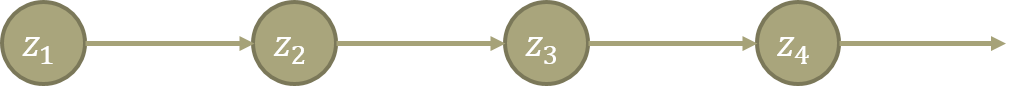
\includegraphics[scale=0.6]{fig10_9.png} 
\caption{1차원 마르코프 연쇄}
\label{fig:10-9}
\end{figure}  

예를 들어, 그림 \ref{fig:10-9}와 같은 형태의 마르코프 연쇄가 주어졌다고 하자. 그러면 $m+1$번째 샘플의 확률 분포는 첫 번째 샘플에서 $m$번째 샘플까지가 조건으로 주어진 경우의 조건부 확률이 된다. 따라서 샘플링 과정에서 $m+1$번째 샘플을 생성할 때는 첫 번째 샘플에서 $m$번째 샘플까지를 참고하게 된다. 그러나 마르코프 연쇄의 성질 중 하나인 무기억성(Memoryless Property)을 적용한다면 확률값을 다음과 같은 형태로 간단하게 나타낼 수 있다. 
\begin{equation}
P(z^{(m+1)} | z^{(1)},\cdots,z^{(m)}) = P(z^{(m+1)} | z^{(m)}), \ m=1,\cdots,M-1
\label{eq:10-12}
\end{equation} 
이것이 바로 마르코프 연쇄를 활용한 잠재 변수에 대해서 그것의 적절한 값을 할당하는 방식이 되겠다.  \\

%슬라이드 16
지금까지 다룬 마르코프 연쇄는 시간의 흐름에 따라서 상태로부터 상태로 변하는 전이 규칙을 전이 행렬 $T$를 통해서 확률적으로 정의하였다. 여기서는 이러한 전이 행렬 $T$로부터 정적 분포 $\pi$를 찾는 것이 중요했다. 반면에 마르코프 연쇄 몬테카를로 방법(Markov Chain Monte Carlo, MCMC)은 정적 분포를 알고 있다고 가정하고 역으로 전이의 흐름을 어떻게 구성할지를 생각한다. 정적 분포 $\pi$에 맞는 샘플링을 진행하기 위해서는 MCMC를 통해서 정적 분포가 사전에 주어진 $\pi$에 부합하도록 전이 행렬을 구성하면서 샘플링을 진행해야 한다.  \\

\begin{figure}[ht] \centering 
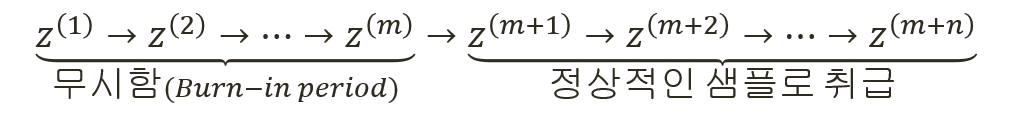
\includegraphics[scale=0.6]{fig10_10.png} 
\caption{마르코프 연쇄 몬테카를로 방법}
\label{fig:10-10}
\end{figure}  

MCMC에서는 우선 주어진 정적 분포 $\pi$와 그때그때 주어지는 현재의 상태에 따른 전이 규칙을 제시한다. 이러한 전이 규칙에 따라 임의의 지점에서 시작해서 시간의 흐름에 따라 상태를 변화시켜 가면서 계속 샘플을 생성한다. 단, 초기에 생성한 몇 개의 샘플은 시작 상태에 영향을 크게 받을 수 있으므로 무시하고 특정 시점 이후의 샘플만을 정식으로 취하는 것이 좋다. \\

%슬라이드 17
\begin{figure}[ht] \centering 
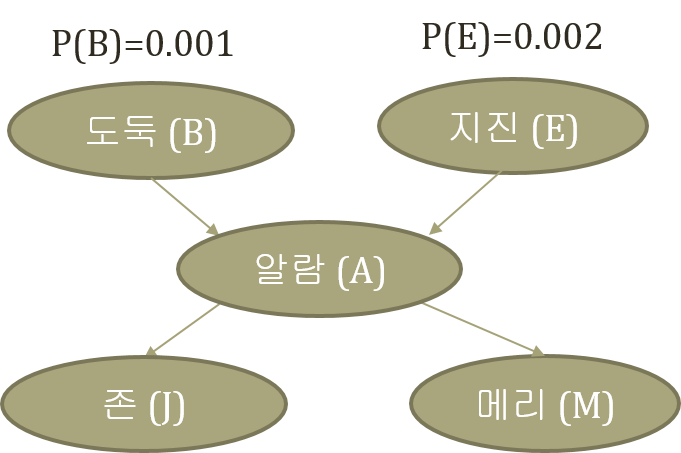
\includegraphics[scale=0.6]{fig10_1.png} 
\caption{베이지안 네트워크 예시}
\label{fig:10-12}
\end{figure}  

MCMC를 이해하기 위해서 chapter 7에서 사용했던 베이지안 네트워크를 대상으로 어떻게 샘플링을 진행할 수 있는지 다시 살펴보도록 하겠다. 그림 \ref{fig:10-12}의 베이지안 네트워크에 따르면 도둑($B$)이 들거나 지진($E$)이 발생했을 때 알람($A$)이 울리며, 알람이 울리면 존($J$)이나 메리($M$)가 나에게 전화를 건다. 하지만 이러한 종류의 사건에는 모두 초기 확률값이나 조건부 확률값이 걸려 있다. 따라서 확률에 따라서는 지진이 발생했는데도 알람이 울리지 않거나, 알람이 울렸는데도 존이 나에게 전화를 하지 않을 수도 있다. 여기서는 알람이 울리지 않았으나 메리는 나에게 전화를 걸었다는 정보가 사전에 주어져 있다고 가정하겠다. 그러면 $A$, $M$ 외에 나머지 알려지지 않은 정보인 $B$, $E$, $J$에 대해서는 우리가 잠재 변수로 취급해야 한다. 그리고 샘플링 과정에서는 모든 샘플에 대해서 $A$에는 false를, $M$에는 true를 할당하고 $B$, $E$, $J$에는 적절한 과정을 통해서 값을 할당해 주어야 한다. 그러나 아직 우리에게는 초기 확률값과 조건부 확률값 외에 어떤 정보도 주어지지 않은 상태이다. \\

\begin{figure}[ht] \centering 
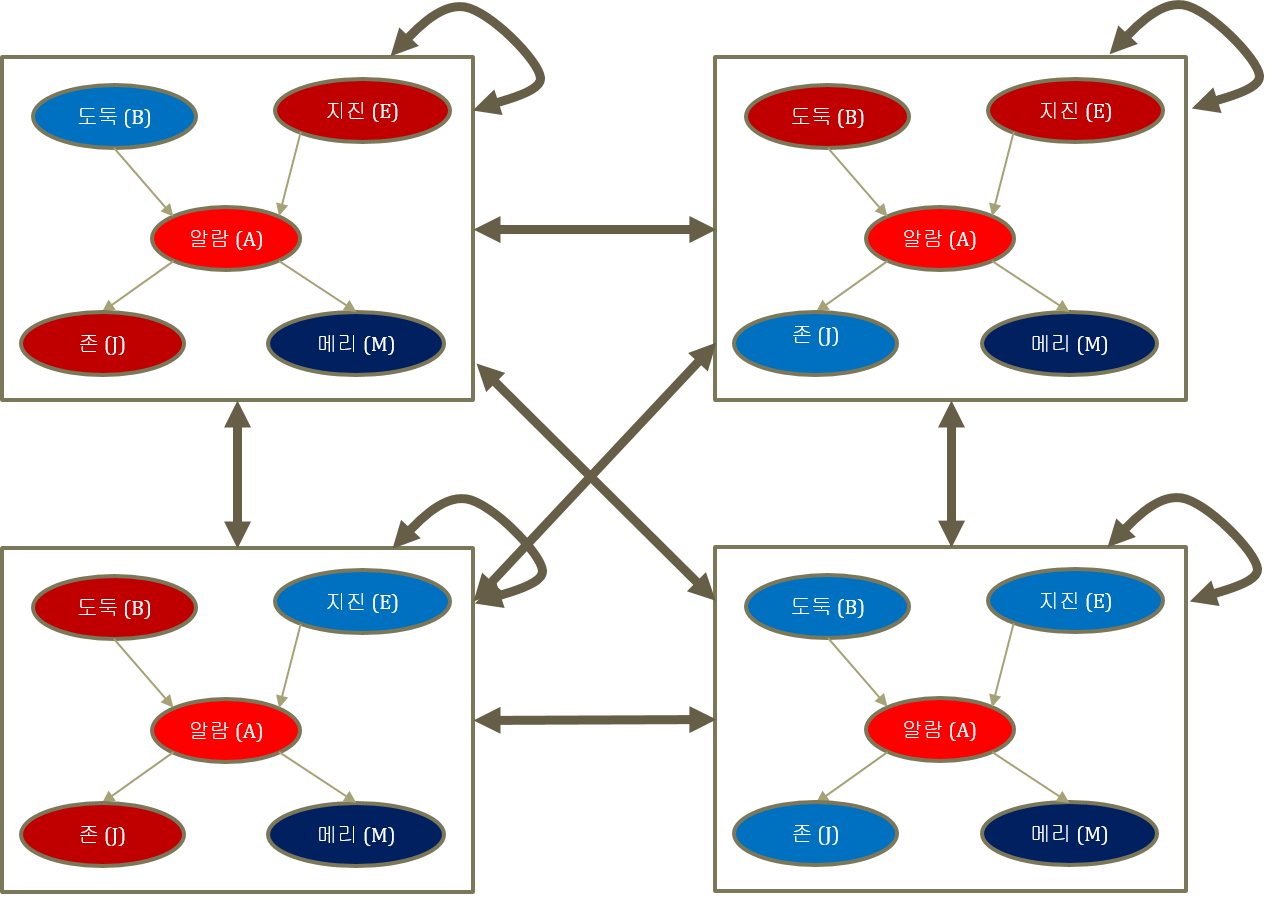
\includegraphics[scale=0.3]{fig10_11.png} 
\caption{마르코프 연쇄 예시}
\label{fig:10-11}
\end{figure}  

여기에 MCMC 샘플링 과정을 적용하려 한다면 제일 먼저 잠재 변수에 아무렇게나 적당한 값을 할당하는 것부터 해야 한다. MCMC에서는 처음 생성되는 몇 개의 샘플을 기각하면서 처음에 아무렇게나 생성한 샘플의 영향을 무시하도록 하는 과정이 있으므로 무작위 생성을 비롯한 적당한 방법으로 이를 생성하면 된다. 여기서는 $B$에 true, $E$에 false, $J$에 false를 할당해 주었다. 그 다음에는 전이 과정을 통해서 알고리즘 상의 전이 규칙에 따른 전이를 계속해서 진행해 준다. 우리가 전체 변수에 대한 특정한 할당을 하나의 상태로 놓았기 때문에 한 번 전이가 일어날때마다 샘플이 하나씩 생성된다. 이러한 마르코프 연쇄에서의 전이와 샘플의 생성이 사전에 정해진 확률값에 의해서 결정되므로 어떤 종류의 샘플은 많이 발생하고 어떤 종류의 샘플은 매우 조금 발생한다. 그러면 개수가 많은 샘플은 개수가 적은 샘플과 비교해서 비교적 적합한 할당이라고 볼 수 있는 것이다. 그 결과로 우리는 샘플링을 통해서 우리가 알지 못했던 잠재 변수에 어떤 식으로 할당해야 적합한 할당이 되는지를 분석할 수 있게 된다.\\

%-----------------------------------------------------------------
\subsection{메트로폴리스-헤이스팅스 알고리즘}
%-----------------------------------------------------------------

%슬라이드 18
정적 분포 $\pi$만이 주어진 상황에서 마르코프 연쇄 기반의 MCMC 샘플링을 진행하기 위해서는 주어진 $\pi$에 맞는 전이 행렬을 구성하는 것이 필수이다. 이를 위한 알고리즘이 바로 메트로폴리스-헤이스팅스 알고리즘(Metropolis-Hastings Algorithm, M-H 알고리즘)이다. \\

우선 M-H 알고리즘이 MCMC의 어떤 부분에서 작동하는지를 알기 위해서 MCMC의 일반적인 알고리즘을 생각해 보도록 하겠다. 먼저 잠재 변수에 대한 현재의 할당이 $z^{t}$로 주어져 있다고 생각해 보자. 그리고  기존의 정보를 활용해서 다음 시점의 할당 후보 $z^{*}$를 제안한다. 이 때 $z^{*}$는 예측 분포(Proposal Distribution)라 불리는 확률 $q(z^{*}|z^{t})$로부터 생성받는다. 여기서 마르코프 연쇄에 대한 정보가 완전하다면 예측 분포 $q$는 전이 행렬과 동일한 개념이 되겠지만 여기서는 어디까지나 임시로 정한 분포일 뿐이다. \\

한편, $q_{t}$로부터 $z^{*}$를 생성했다고 하더라도 그것이 바로 다음 시점의 할당인 $z^{t+1}$이 되는 것은 아니다. 여기에는 따로 수용 확률(Acceptance Probability) $\alpha$가 있어서 $\alpha$의 확률로 $z^{*}$를 취하거나 $1-\alpha$의 확률로 $z^{*}$를 버리는 과정을 거쳐야 한다. 실제 알고리즘에서는 0에서 1 사이의 실수값을 가지는 균일 분포에서 무작위로 값을 하나 생성해서 이것이 $\alpha$보다 작거나 같다면 $z^{t+1}=z^{*}$로, $\alpha$보다 크다면 $z^{t+1}=z^{t}$로 정하는 식으로 이를 구현한다. 여기까지의 과정을 계속해서 반복하는 것이 바로 MCMC의 일반적인 과정이다. \\

이제 M-H 알고리즘에 대해서 본격적으로 알아보도록 하자. 우리에게 주어진 것으로는 먼저 잠재 변수의 할당에 대한 확률 밀도 함수 $P$가 있다. 그리고 우리가 임의로 정할 수 있는 예측 분포 $q$가 있다. 우리는 임의로 정한 $q$가 균형 방정식을 따르는지를 확인해야 한다. 이는 $q(z^{t}|z^{*})P(z^{*})$와 $q(z^{*}|z^{t})P(z^{t})$가 같은지의 여부를 확인하는 것과 같다. 이것을 확인할 수 있도록 비율 $r$을 정의하도록 하겠다.
\begin{equation}
r(z^{*}|z^{t}) = \frac{q(z^{t}|z^{*})P(z^{*})}{q(z^{*}|z^{t})P(z^{t})}
\label{eq:10-13}
\end{equation} 
이 식이 1에 가까우면 가까울수록 예측 분포 $q$는 균형 방정식을 따르는 것이 된다. \\

한편으로 어째서 $q$가 균형 방정식을 따르는지를 확인해야 하는 것일까? MCMC는 주어진 정적 분포 $\pi$로부터 알맞은 전이 규칙을 찾기 위해서 역산하는 과정이 된다. 다시 말해서 MCMC의 결과로부터 다시 정적 분포 $\pi$를 산출할 수 있어야 한다는 것이다. 이를 위해서 생각해야 할 것이 바로 가역 마르코프 연쇄이다. 전이 규칙 $T$와 정적 분포 $\pi$를 가지는 가역 마르코프 연쇄에서는 임의의 상태 $i$, $j$에 대해서 $\pi_{i}T_{i,j}$와 $\pi_{j}T_{j,i}$가 같아야 한다. 또한, 임의의 분포 $\pi$가 있어서 가역 성질을 만족한다면 $\pi$는 자동으로 정적 분포가 된다. 따라서 $\pi_{i}T_{i,j}$와 $\pi_{j}T_{j,i}$가 일치하는지의 여부를 확인하는 것으로 $T$와 $\pi$가 각각 알맞은 전이 행렬과 정적 분포인지를 확인할 수 있다. 이런 관점에서 비율 $r$이 1과 같다면 $q$가 올바른 전이 규칙이라고 생각할 수 있는 것이다. \\

또한, 여기서의 $r$은 $q$가 얼마나 적합한지를 확인하는 용도 외에 $q$를 교정하는 데에도 사용한다. 원래의 $q$는 정의하기에 따라서 가역 마르코프 연쇄가 아닐 수도 있다. 비율 $r$은 이러한 $q$를 가역 마르코프 연쇄에 가깝게 되도록 교정하는 역할을 한다. 어떻게 교정이 이루어지는지를 확인하기 위해서 $r(z^{*}|z^{t})$가 1보다 작은 경우와 1보다 큰 경우에 대해서 각각을 따로 생각해 보겠다. 먼저 $r(z^{*}|z^{t})$이 1보다 작은 경우를 생각해 보자. 이는 $q(z^{t}|z^{*})P(z^{*})$가 $q(z^{*}|z^{t})P(z^{t})$보다 작다는 것과 같은 말이다. 따라서 $q(z^{t}|z^{*})$를 키우고 $q(z^{*}|z^{t})$를 줄이는 방향으로 교정이 이루어져야 한다. 여기서는 $q(z^{t}|z^{*})$는 그대로 유지하고 $q(z^{*}|z^{t})$에 $r(z^{*}|z^{t})$을 곱해서 $q(z^{*}|z^{t})$의 값을 줄여나갔다. 다음으로 $r(z^{*}|z^{t})$이 1보다 큰 경우를 생각해 보자. 이번에는 $q(z^{t}|z^{*})P(z^{*})$가 $q(z^{*}|z^{t})P(z^{t})$보다 크기 때문에 $q(z^{t}|z^{*})$를 줄이고 $q(z^{*}|z^{t})$를 키우는 방향으로 교정이 이루어져야 한다. 여기서는 $q(z^{*}|z^{t})$는 그대로 유지하고 $q(z^{t}|z^{*})$에 $r(z^{t}|z^{*})$을 곱해서 $q(z^{*}|z^{t})$의 값을 줄여나갈 수 있다. \\

이러한 과정에서 $q(z^{*}|z^{t})$에는 $1$이나 $r(z^{*}|z^{t})$가 곱해지게 된다. 여기서는 $r(z^{*}|z^{t})$이 1보다 작은 경우에만 $r(z^{*}|z^{t})$을 곱하고 그 외에는 $1$을 곱한다. 따라서 수용 확률 $\alpha(z^{*}|z^{t})$는 $1$과 $r(z^{*}|z^{t})$ 중에서 더 작은 값이 된다. 다시 말해, $\alpha(z^{*}|z^{t})=\textrm{min} \{ 1, r(z^{*}|z^{t}) \}$이다. MCMC 과정으로 돌아와서 이것이 어떤 의미를 가지는지를 생각해보면, $z^{t}$에서 $z^{*}$로 가는 샘플 중에서 일부를 $\alpha(z^{*}|z^{t})$의 확률로 수용하고 $1-\alpha(z^{*}|z^{t})$의 확률로 기각하는 것과 같다. 따라서 전체에서 해당 샘플의 양은 $\alpha(z^{*}|z^{t})$의 비율로 줄어들게 되어 이는 $q(z^{*}|z^{t})$을 조절한 것과 같게 된다. 이런 식으로 예측 분포 $q$가 잘 정의되지 않았을 때에도 수용 확률 $\alpha$를 구하고, 이를 활용해서 균형 방정식을 만족하는 가역 마르코프 연쇄를 만들어 줄 수 있다. 그리고 생성한 마르코프 연쇄에서 상태의 전이를 계속해서 반복하다 보면 결국에는 분포가 사전에 주어진 정적 분포로 수렴하게 된다. \\

%슬라이드 19
이제 M-H 알고리즘을 조금 더 직관적인 관점에서 이해해 보자. M-H 알고리즘은 MCMC라는 확률적 전이를 알아보는 것과 같다. 따라서 이번에는 전이 행렬 $T$의 관점에서 M-H 알고리즘을 생각해 보겠다. 먼저 현재 상태인 $z^t$가 있고 비교할 상대인 예측 분포 $z^{*}$가 있다고 하자. 그러면 M-H 알고리즘 상에서 전이 행렬 $T_{t,*}^{MH}$를 $q(z^{*}|z^{t})$와 $\alpha(z^{*}|z^{t})$의 곱으로 나타낼 수 있다. 이런 식으로 정의한 전이 확률은 균형 방정식을 만족시키며, 따라서 이것은 정적 분포가 된다. 또한, $P(z)$를 계산하는 것이 어렵지 않다면 우리는 $\alpha(z^{*}|z^{t})$값을 다음과 같이 계산할 수 있다. 
\begin{equation}
\alpha(z^{*}|z^{t}) = \textrm{min} \{ 1, \frac{q(z^{t}|z^{*})P(z^{*})}{q(z^{*}|z^{t})P(z^{t})} \}
\label{eq:10-20}
\end{equation} 
여기서 예측 분포 $q$를 어떻게 정할 것인지를 생각해야 하며, $q(z^{*}|z^{t})$를 어떻게 잡느냐에 따라서 M-H 알고리즘의 종류가 결정된다. 이 때, $q(z^{*}|z^{t})$을 정하는 방법으로 랜덤 워크(Random Walk)가 있다. 랜덤 워크를 M-H 알고리즘에 적용하는 것은 간단하다. 먼저 평균이 $z^{t}$, 분산이 $\sigma^2$인 정규 분포로부터 수를 하나 생성해서 $z^{*}$로 정한다. 그리고 이것을 기각할지의 여부를 확률적으로 결정한다. 여기서는 $q$를 정규 분포의 확률 밀도 함수로 정했기 때문에 다음의 확률로 $z^{*}$를 받아들이게 된다. 
\begin{equation}
q(z^{*}|z^{t}) = \frac{1}{\sigma \sqrt{2 \pi}} \textrm{exp} (-\frac{(z^{*}-z^{t})^{2}}{2\sigma^2})
\label{eq:10-21}
\end{equation}
여기서의 전이 행렬은 앞에서처럼 $q(z^{*}|z^{t})$와 $\alpha(z^{*}|z^{t})$의 곱이 된다. 이렇게 랜덤 워크를 활용한 M-H 알고리즘에서 전이란 정규 분포를 근거로 이루어지게 된다. \\

%슬라이드 20
\begin{figure}[ht] \centering 
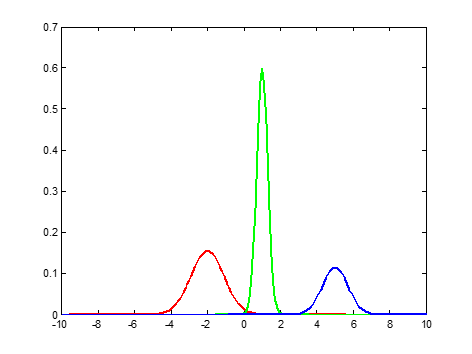
\includegraphics[scale=0.7]{fig10_22.png} 
\caption{가우시안 혼합 분포 예시}
\label{fig:10-11-1}
\end{figure}  

다음은 랜덤 워크를 활용한 M-H 알고리즘을 구현해서 실험을 진행한 결과이다. 실험 대상이 되는 분포는 앞에서 사용한 봉우리가 세 개 있는 형태의 가우시안 혼합 분포이다. 우리는 이러한 분포로부터 샘플링을 해서 M-H 알고리즘의 실제 결과를 알아보고자 한다. 그러나 세 번의 실험에 대해서 랜덤 워크의 평균값은 세 경우 모두 $2.0$으로 일정하게 정하였으나, 랜덤 워크의 분산은 각각 $0.1$, $1.0$, 그리고 $40$으로 서로 다르게 정해서 실험을 진행하였다. 우리가 확인해야 할 것은 영점에서 시작해서 얼마나 많은 이동이 이루어졌는가이다. \\

\begin{figure}[ht] \centering 
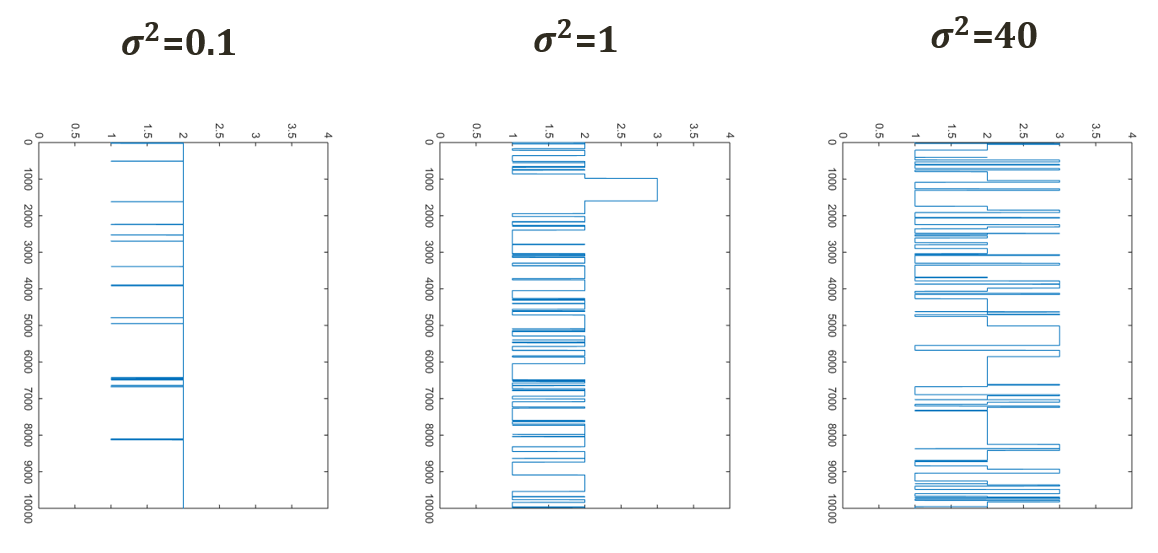
\includegraphics[scale=0.6]{fig10_24.png} 
\caption{잠재 변수에 대한 선택 샘플링 결과}
\label{fig:10-11-3}
\end{figure}  

\begin{figure}[ht] \centering 
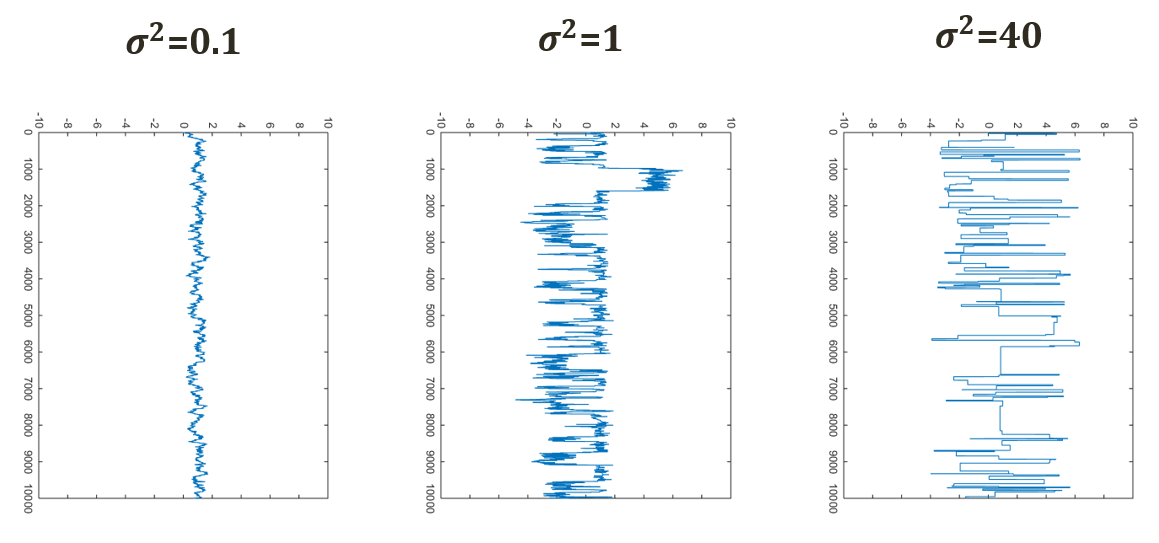
\includegraphics[scale=0.6]{fig10_25.png} 
\caption{관찰 변수에 대한 샘플링 결과}
\label{fig:10-11-4}
\end{figure}  

랜덤 워크의 폭은 전적으로 분산에 의해서 결정되므로 분산이 작은 경우에는 이동이 덜 일어나지만 분산이 큰 경우에는 이동이 매우 자주 일어나게 된다. 그림 \ref{fig:10-11-3}의 잠재 변수 $z$에 대한 선택 샘플링 결과와 그림 \ref{fig:10-11-4}의 관찰 변수 $x$에 대한 샘플링 결과를 보면 이러한 경향을 분명히 확인할 수 있다. 

\begin{figure}[ht] \centering 
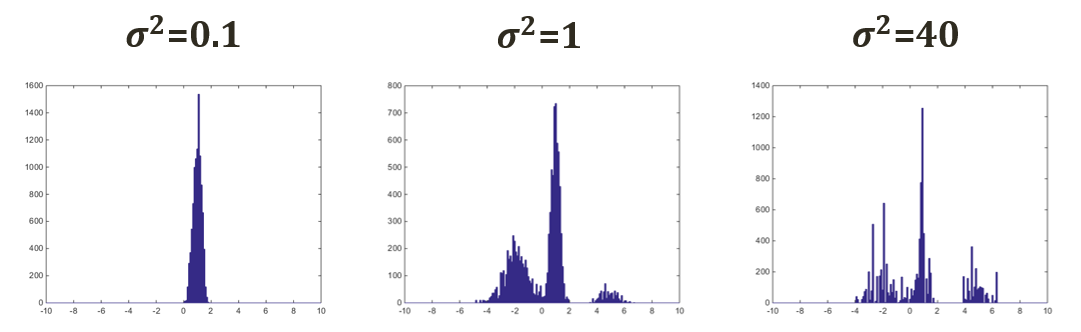
\includegraphics[scale=0.6]{fig10_23.png} 
\caption{랜덤 워크를 활용한 M-H 알고리즘의 샘플링 결과}
\label{fig:10-11-2}
\end{figure}  

그리고 이렇게 샘플링을 진행해서 그래프로 나타낸 것이 바로 그림 \ref{fig:10-11-2}이다. 먼저 분산이 $0.1$인 경우에는 원래의 그래프에서 가운데 부분만 정밀하게 샘플링이 되어 있으며, 다른 부분은 전혀 샘플링이 되어있지 않는다는 것을 확인할 수 있다. 이것은 랜덤 워크의 범위가 제한되어 있기 때문에 $x=2$ 부근에 위치한 봉우리에 해당하는 $z$에 대해서만 샘플링이 잘 되고 있기 때문이다. 그리고 $x=2$에서 멀리 벗어나 있는 봉우리의 $z$는 샘플링이 잘 되지 않고 있다. 실제로 그림 \ref{fig:10-11-3}과 그림 \ref{fig:10-11-4}의 분산이 $0.1$인 경우의 그래프에서는 $z$의 변화가 거의 일어나지 않고 있으며, $x$값 또한 특정 범위 내에 머물러 있다는 것을 확인할 수 있다. \\

이것을 극복하기 위해서 분산을 $1.0$으로 늘려주면 혼합 모델의 세 개의 봉우리가 모두 드러나게 된다. 그리고 그림 \ref{fig:10-11-3}과 그림 \ref{fig:10-11-4}을 보면 아까의 경우와는 달리 $z$값이 비교적 많이 변하고 있으며, $x$값은 특정 범위에서 머물지 않고 시간의 흐름에 따라 계속해서 다른 값을 나타내고 있다는 것을 확인할 수 있다. 따라서 분산을 크게 만들어 좀 더 넓은 범위에서 샘플링을 진행한다면 전체적인 히스토그램을 그리기에 좋다는 것을 알 수 있다. 그러나 그래프의 정밀함은 첫 번째와 비교해서 조금 떨어지며, 여전히 세 번째 봉우리에 대해서는 제대로 감지를 하지 못 하고 있는 상황이다. \\ 

이전 결과에서 제대로 샘플링하지 못했던 세 번째 봉우리까지 제대로 샘플링하기 위해서 세 번째 실험은 분산을 $40.0$으로 크게 늘여서 진행하였다. 그러면 예상한 것과 같이 이번에는 세 번째 봉우리도 잘 샘플링을 할 수 있게 된다. 이는 분산이 매우 크기 때문에 $z$의 변동성이 훨씬 커지게 되어 세 번째 봉우리로 더욱 잘 이동하게 되었기 때문이다. 그러나 그래프의 정밀함은 이전에 비해서 더욱 떨어졌다는 것을 확인할 수 있다. 따라서 랜덤 워크를 활용한 M-H 알고리즘으로 샘플링을 할 때에는 랜덤 워크의 분산을 처음에는 넓게 잡아서 전체적인 형태를 만든 뒤에, 분산을 점차 줄여나가면서 개별적으로 정밀한 샘플링을 하는 식으로 진행해 나가야 한다. \\


%-----------------------------------------------------------------
\subsection{깁스 샘플링}
%-----------------------------------------------------------------

%슬라이드 21
깁스 샘플링(Gibbs Sampling)은 미국의 물리학자인 조사이어 윌러드 기브스(Josiah Willard Gibbs, 1839-1903)가 창안한 샘플링 방법이다. 앞에서 설명한 M-H 알고리즘에서는 예측 분포 $q$와 수용 확률 $\alpha$를 사용해서 전이 행렬을 구성하였다. 깁스 샘플링은 기존에 있던 확률 밀도 함수로부터 예측 분포 $q$를 정해서 전이 행렬을 구성하는 M-H 알고리즘의 특수한 경우를 말한다. \\

먼저 특정 시점에서 잠재 변수에 대한 할당이 $z^{t}=(z^{t}_{k}, z^{t}_{-k})$와 같이 주어져 있다고 하자. 여기서 $z^{t}_{k}$는 한 개의 특정 잠재 변수에 대한 할당을, $z^{t}_{-k}$는 나머지 잠재 변수에 대한 할당을 의미한다. 그러면 깁스 알고리즘 과정에서 다음 시점에 대한 새로운 할당은 $z^{*}=(z^{*}_{k}, z^{t}_{-k})$와 같이 주어지게 된다. 다시 말해, 시간이 한 번 바뀔때마다 정확히 하나의 잠재 변수에 대한 할당만 갱신되는 것이다. 여기서 확률 밀도 함수를 활용해서 예측 분포 $q(z^{*}|z^{t})$를 $P(z^{*}|z^{t}_{-k})$와 같이 정하였다. 그러면 $q$는 $P(z^{*}_{k}, z^{t}_{-k}|z^{t}_{-k})$이므로 결국 $P(z^{*}_{k}|z^{t}_{-k})$와 같게 된다. 이것은 $k$번째 잠재 변수 외 나머지 잠재 변수의 할당이 주어진 상황에서 $k$번째 잠재 변수의 알맞은 할당이 무엇인지를 생각하는 것과 같게 된다. \\

이제 이런 식으로 $q$를 정했을 때 과연 이것이 균형 방정식을 만족하는지를 살펴보도록 하겠다. 균형 방정식에 따르면 $P(z^{t})q(z^{*}|z^{t})$와 $P(z^{*})q(z^{t}|z^{*})$는 정확히 일치해야 한다. 다음의 전개 과정은 두 식이 일치한다는 것을 명확하게 보여준다.   
\begin{eqnarray}
P(z^{t})q(z^{*}|z^{t}) & = & P(z^{t}_{k}, z^{t}_{-k}) P(z^{*}_{k} | z^{t}_{-k}) \nonumber \\
& = & P(z^{t}_{k}| z^{t}_{-k}) P(z^{t}_{-k}) P(z^{*}_{k} | z^{t}_{-k}) \nonumber \\
& = & P(z^{t}_{k}| z^{t}_{-k}) P(z^{*}_{k}, z^{t}_{-k}) \nonumber \\
& = & q(z^{t}|z^{*}) P(z^{*}) \label{eq:10-30}
\end{eqnarray} 
우리는 이러한 전개 과정에서 결합 확률과 조건부 확률 사이의 관계를 활용하였다. 따라서 $q(z^{*}|z^{t}) = P(z^{*}|z^{t}_{-k})$는 균형 방정식을 만족시키며, 수용 확률 $\alpha$의 값은 언제나 $1$이 된다.  \\

\begin{figure}[ht] \centering 
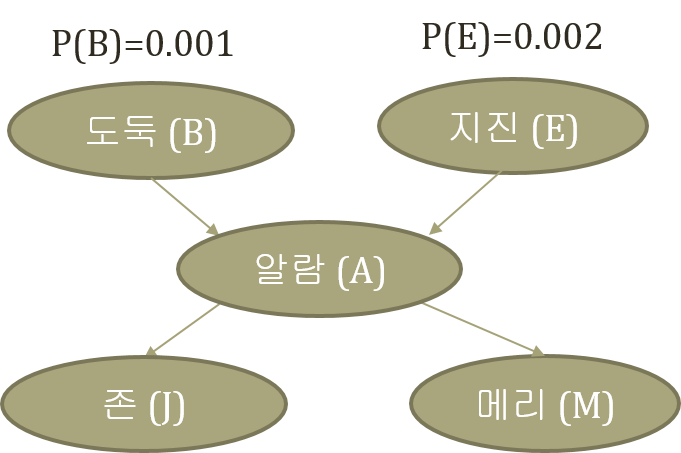
\includegraphics[scale=0.6]{fig10_1.png} 
\caption{베이지안 네트워크 예시}
\label{fig:10-12-1}
\end{figure}  

\begin{figure}[ht] \centering 
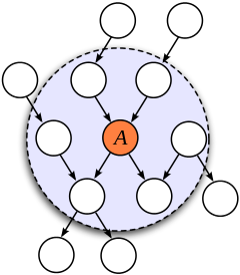
\includegraphics[scale=0.6]{fig10_12.png} 
\caption{마르코프 블랭킷}
\label{fig:10-13}
\end{figure}  

이제 앞에서 사용했던 예제를 통해서 깁스 샘플링을 자세히 알아보도록 하겠다. 여기서는 $A$에 false가, $M$에 true가 할당되었다고 가정하겠다. 그러면 깁스 샘플링을 통해서 나머지 잠재 변수에 대한 할당을 진행할 수 있다. 깁스 샘플링을 진행하기 위해서 제일 먼저 해야 할 것은 잠재 변수에 임의로 값을 할당하는 것이다. 여기서는 $B$, $E$, $J$에 각각 true, true, true를 할당해 주었다. 다음으로 잠재 변수 중 하나를 선택해서 그 값을 갱신해 준다. 여기서는 $B$를 선택하였다. 한편, $A$와 $E$의 값이 고정되어 있을 때 $B$와 $M$, $J$ 사이에는 아무런 관계가 없다. 그러면 우리는 조건부 확률을 구할 때 마르코프 블랭킷의 바깥에 있는 변수에는 신경 쓸 필요가 없다는 사실을 활용해서 확률 계산을 간단히 수행할 수 있다. 이에 따르면 우리는 $A$가 false, $E$가 true일 때 $B$가 true일 확률을 구하고 이러한 확률에 따라서 $B$의 할당값을 생성하면 된다. 여기서는 $B$에 false를 새로 할당했다고 하겠다. 그러면 이전 M-H 알고리즘에서는 수용 확률을 따로 계산해서 $B$에 false를 할당하는 것을 확정지을지의 여부를 확률적으로 결정하는 과정을 거쳐야 한다. 그러나 깁스 샘플링에서는 수용 확률이 $1$이므로 $B$에 할당한 false를 그대로 확정지으면 된다. 다음으로 잠재 변수 중에서 $J$를 선택하고 $J$가 true일 확률을 생각해야 한다. 여기서는 마르코프 블랭킷 내부에 있는 $A$만을 생각해서 $A$가 false인 경우에서 $J$의 조건부 확률값을 가져온다. 그러고 나서 조건부 확률을 바탕으로 무작위로 $J$에 값을 할당한다. 마지막으로 잠재 변수 중에서 $E$를 선택했을 경우에는 $A$와 $B$만을 생각해서 확률값을 구하고, 이렇게 구한 확률에 따라서 무작위로 $E$에 값을 할당하면 된다. 이런 식으로 잠재 변수인 $A$, $B$, $E$ 중에서 하나만을 선택해서 나머지가 특정 값으로 고정된 채로 선택한 변수 하나만을 바꾸는 과정을 반복해서 진행하는 것이 바로 깁스 샘플링의 과정이 된다. \\

%슬라이드 22, 23
\begin{figure}[ht] \centering 
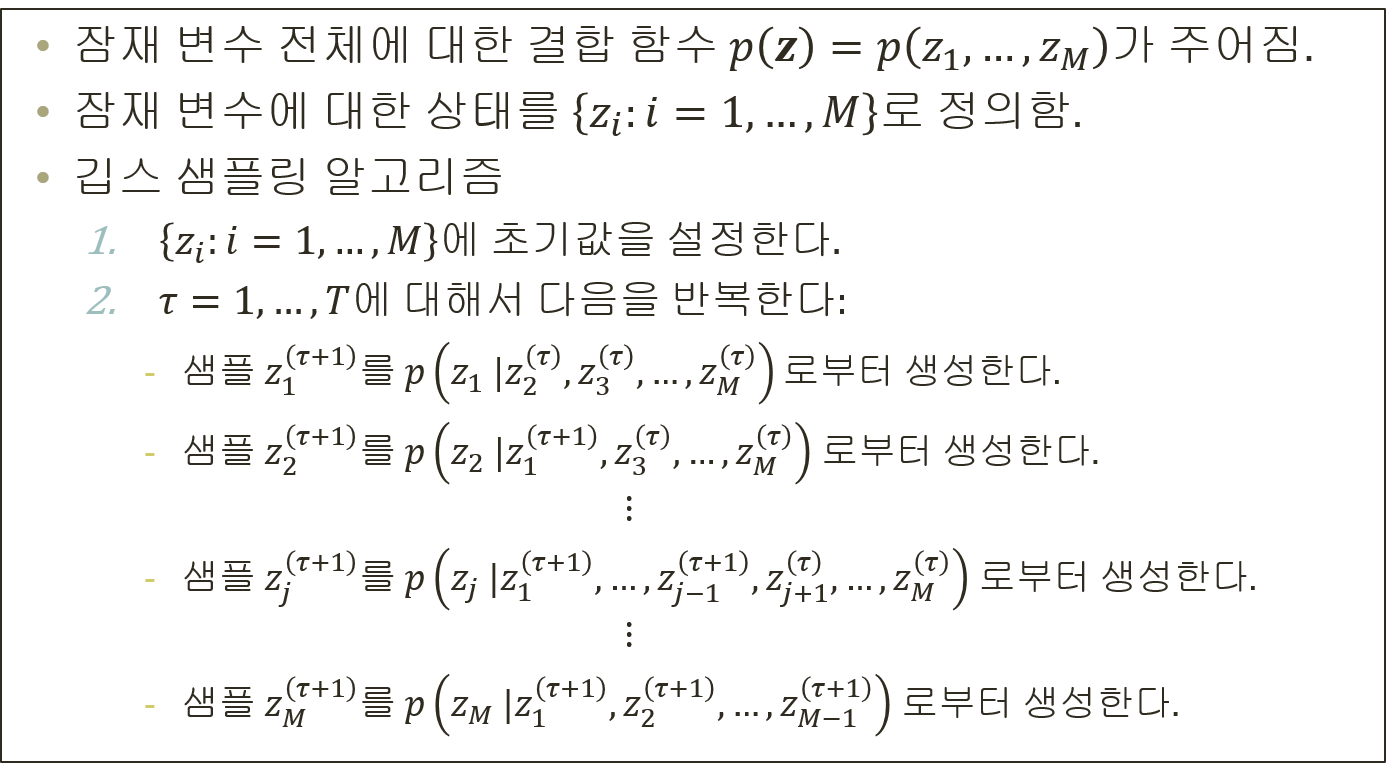
\includegraphics[scale=0.45]{fig10_17.png} 
\caption{전체 깁스 샘플링 과정}
\label{fig:10-18}
\end{figure}

\begin{figure}[ht] \centering 
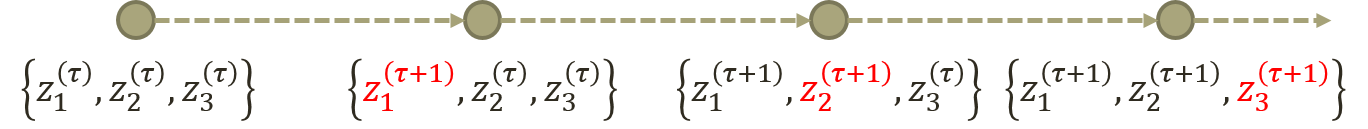
\includegraphics[scale=0.5]{fig10_13.png} 
\caption{세 잠재 변수에서의 깁스 샘플링 과정}
\label{fig:10-14}
\end{figure}

그림 \ref{fig:10-18}에서 이러한 깁스 샘플링의 과정을 설명하고 있다. 여기서 한 번의 반복은 하나의 잠재 변수 값을 갱신하는 과정이 된다. 세 개의 잠재 변수 $z_1$, $z_2$, $z_3$와 결합 확률 $p(z_1, z_2, z_3)$가 주어졌다고 하자. 그러면 현재 시점에서의 $z_2^{\tau}$, $z_3^{\tau}$를 바탕으로 $z_1$에 할당할 수 있는 값에 대한 확률 분포인 $p(z_1 | z_2^{\tau}, z_3^{\tau})$를 바탕으로 무작위로 $z_1^{\tau+1}$을 생성한다. 그리고 이렇게 생성한 $z_1^{\tau+1}$를 다음부터 사용하게 된다. 다음으로 $z_2$에 대해서 $z_1^{\tau+1}$과 $z_3^{\tau}$가 주어져 있을 때 $z_2$에 대한 확률 분포인 $p(z_2 | z_1^{\tau+1}, z_3^{\tau})$를 바탕으로 $z_2^{\tau+1}$를 생성한다. 마찬가지로 $z_3$에 대해서도 $z_1^{\tau+1}$과 $z_2^{\tau+1}$를 바탕으로 확률 분포 $p(z_3 | z_1^{\tau+1}, z_2^{\tau+1})$를 구성하고 이를 바탕으로 $z_3^{\tau+1}$를 생성한다. 이런 식으로 $z_1$, $z_2$, $z_3$를 차례대로 갱신해 주는 것이 깁스 샘플링의 과정이 된다.\\

\begin{figure}[ht] \centering 
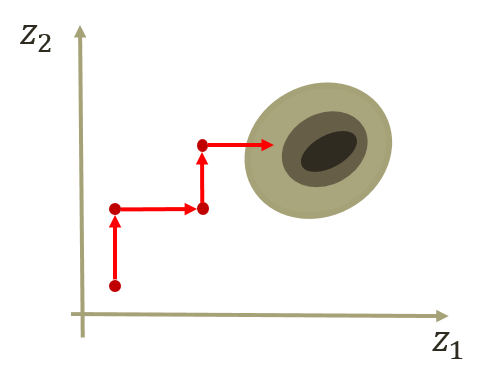
\includegraphics[scale=0.8]{fig10_14.png} 
\caption{두 잠재 변수에서의 깁스 샘플링 과정}
\label{fig:10-15}
\end{figure}

깁스 샘플링의 과정을 시각적으로 확인하기 위해서 이제 두 개의 잠재 변수를 가진 확률 모델에서의 깁스 샘플링 과정을 생각해 보겠다. 여기에는  $z_1$과 $z_2$만이 있다. 우리는 그림 \ref{fig:10-15}의 그래프에서 적합도가 특별히 높은 지점을 확인할 수 있다. 그러나 깁스 샘플링을 시작할 때에는 이것을 모르고 있으므로 처음에는 적당히 정한 임의의 지점에서 시작해야 한다. 그 지점에서 $z_1$이 고정된 값이라고 생각하고 적절한 $z_2$를 찾아서 이동하는 식으로 샘플링을 진행한다. 그 다음에는 아까의 $z_2$가 고정된 값이라고 생각하고 $z_1$의 값을 갱신한다. 이러한 과정을 반복하면서 적합한 지점으로 계속해서 이동하면서 샘플링을 진행하게 된다. 깁스 샘플링은 이런 식으로 마르코프 연쇄 과정을 통해서 적절한 지점으로 이동하면서 샘플링을 진행하게 된다. \\

%슬라이드 24
\begin{figure}[ht] \centering 
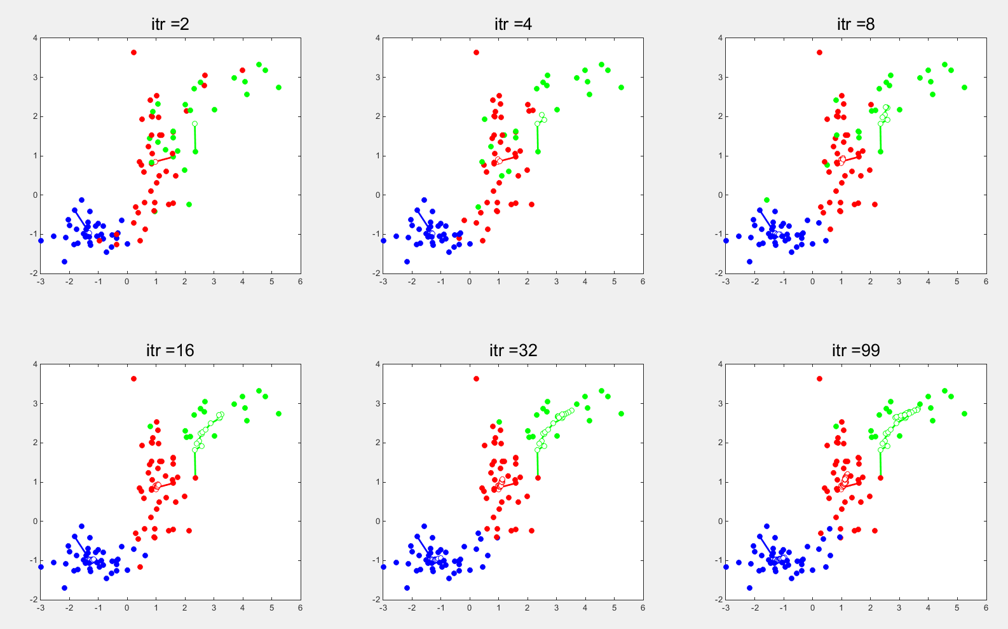
\includegraphics[scale=0.6]{fig10_15.png} 
\caption{깁스 샘플링 결과}
\label{fig:10-16}
\end{figure}

큰 의의가 있는 것은 아니지만 의외로 깁스 샘플링을 가우시안 혼합 모델에도 적용할 수 있다. 앞서 chapter 8에서 설명한 k-평균 군집화나 가우시안 혼합 모델을 사용하는 EM 알고리즘에서는 잠재 변수 $z$에 적합한 할당을 하기 위해서 $p(z|\cdot)$가 가장 크게 되는 최적의 $z$를 찾아서 할당해 주었다. 깁스 샘플링을 활용한다면 최적화 기반의 방법 대신 $p(z|\cdot)$를 바탕으로 확률적으로 $z$를 할당할 수 있다. 이러한 샘플링 기반의 할당 방법은 개별 데이터 포인트마다 알맞는 군집을 할당해주는 것이 되기 때문에 강한 군집화의 하나인 것처럼 보인다. 그림 \ref{fig:10-16}의 그래프는 이를 잘 보여준다. 실제로 깁스 샘플링 기반의 군집화를 진행한다면, 처음에는 서로 다른 색의 데이터 포인트가 여기저기 흩어져 있는 것을 확인할 수 있다. 그러나 계속해서 샘플링 과정을 반복한다면 우리가 군집화 알고리즘에 기대했던 분명한 군집화 결과가 나타나게 된다. \\

\begin{figure}[ht] \centering 
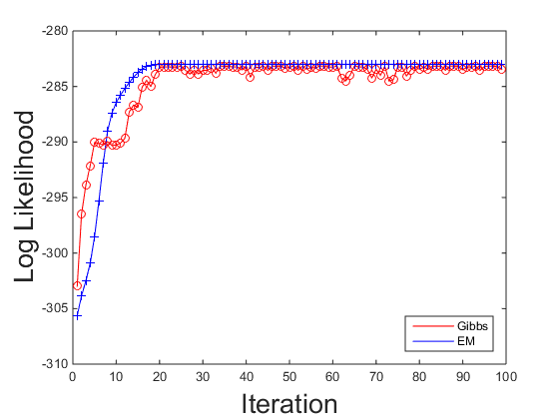
\includegraphics[scale=0.8]{fig10_16.png} 
\caption{EM 알고리즘과 깁스 샘플링 기반의 군집화 비교}
\label{fig:10-17}
\end{figure}

그림 \ref{fig:10-17}의 그래프는 EM 알고리즘과 깁스 샘플링 기반의 군집화에 대해서 군집화가 얼마나 잘 이루어졌는지를 나타내어 준다. 그래프에서 가로축은 군집화의 반복 횟수, 세로축은 로그 우도 값을 나타낸다. 그래프를 보면 EM 알고리즘에서는 반복이 늘어나면 늘어날수록 로그 우도 값이 좋아지는 것을 확인할 수 있다. 반면에 깁스 샘플링을 이용한 군집화에서는 수렴 속도가 일정하지 않으며 몇몇 구간에서는 오히려 로그 우도 값이 나빠지는 것을 확인할 수 있다. 이것은 깁스 샘플링을 이용한 군집화는 EM 알고리즘과 같은 최적화의 관점에서 작동하는 군집화가 아니기 때문이다. \\

그럼에도 불구하고 어떤 경우에는 깁스 샘플링 기반의 군집화가 더 정확하고 좋을 수 있다. EM 알고리즘에 찾는 최적해는 전역 최적해가 아닌 어디까지나 지역 최적해에 불과하며, 때로는 알고리즘의 진행 과정에서 안장점에 빠질 수도 있기 때문이다. 하지만 샘플링에 기반한 군집화에서는 지역해에서 벗어날 수 있는 여지가 다소나마 존재하며, 그 때문에 시간이 충분히 주어진다면 MCMC 및 깁스 샘플링 기반의 군집화가 더 나은 결과를 보일 수도 있다. \\

하지만 일반적으로 빠른 시간 내로 최적의 결과를 내놓을 수 있는 EM 알고리즘이 현실에서는 잘 쓰인다. 이러한 EM 알고리즘 기반의 군집화 및 추정 기법을 좀 더 발전시킨 것으로 변화 추정(Variational Inference)이라는 것이 있다. 현실에서는 쓰이는 알고리즘은 문제의 유형에 따라 변화 추정이나 깁스 샘플링 기반의 추정을 사용한다. 그리고 뒤에서 다룰 잠재 디리클레 할당에서도 깁스 샘플링 기반 추정이 쓰인다. \\

%-----------------------------------------------------------------
\section{잠재 디리클레 할당}
%-----------------------------------------------------------------

%-----------------------------------------------------------------
\subsection{토픽 모델링}
%-----------------------------------------------------------------

%슬라이드 25
이제는 토픽 모델링과 같은 분야에서 나오는 복잡한 베이지안 네트워크의 파라미터 추정에 적용할 수 있는 잠재 디리클레 할당에 대해서 알아보고자 한다. 여기서 잠재 디리클레 할당은 샘플링 기반 추론의 하나이며, 파라미터를 추정하는데 지난번까지 다룬 깁스 샘플링을 적용하는 방법이 된다. 특히 잠재 디리클레 할당을 위한 깁스 샘플링으로 특별히 붕괴 깁스 샘플링이 있으며 여기서는 그것 또한 자세히 다루고자 한다. \\

%슬라이드 26
\begin{figure}[ht] \centering 
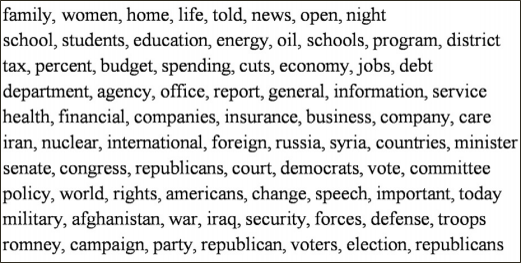
\includegraphics[scale=0.7]{fig10_18.png} 
\caption{신문 기사에서 추출한 핵심 단어 목록}
\label{fig:10-18-1}
\end{figure}

먼저 잠재 디리클레 할당을 적용할 수 있는 대표적인 사례인 토픽 모델링에 대해서 간단히 짚어보도록 하겠다. 토픽 모델링(Topic Modeling)은  글의 단어들을 비슷한 의미를 가진 것들끼리 군집화하면서 기계 학습의 방법론으로 글의 주제를 파악하도록 하는 텍스트마이닝의 한 방법이다. 여기서는 간단한 예시를 하나 들어서 토픽 모델링을 이해할 수 있는 기회를 가지도록 하겠다. \\

그림 \ref{fig:10-18-1}은 토픽 모델링의 예제로서 Obama(버락 오바마 전 미국 대통령)와 관련해서 신문에서 보도한 여러 개의 기사로부터 추출한 단어가 차례대로 나열되어 있다. 그러나 이러한 단어들은 무작위로 나열되어 있는 것이 아니며, 같은 기사에서 나온 것끼리는 나름대로의 규칙과 패턴이 있다. 먼저 첫 번째 기사에서는 family(가족), women(여성), home(가정), ..., night(밤) 등의 단어를 찾을 수 있었다. 이로부터 우리는 첫 번째 기사가 여성, 가족에 관련된 주제의 글이라고 추측할 수 있다. 한편, 마지막 기사에서는 romney(롬니), campaign(운동), party(정당), ..., republicans(공화당원) 등의 단어를 찾을 수 있었다. 그러면 마지막 기사는 미국 대선을 다루고 있다고 생각할 수 있다. 같은 식으로 뒤에서 두 번째 기사에는 military(군사), afghanistan(아프가니스탄), war(전쟁), ..., troops(병력) 등의 단어가 있는 것으로 보아 아프가니스탄 전쟁을 다루는 글이라고 추측할 수 있다. 이런 식으로 주어진 10개의 기사들은 각각 주제를 하나씩 가지고 있다. \\

\begin{figure}[ht] \centering 
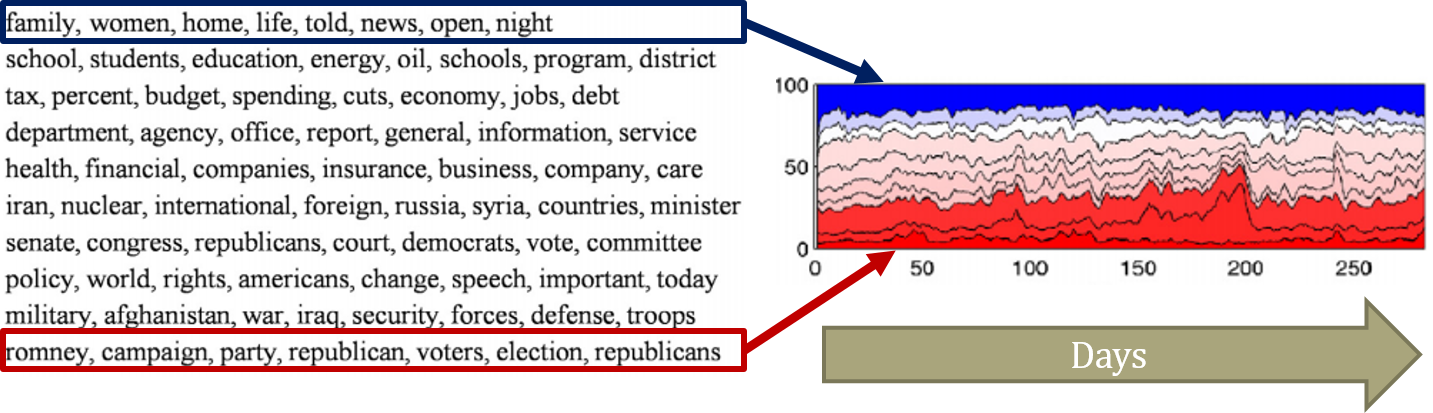
\includegraphics[scale=0.5]{fig10_19.png} 
\caption{토픽 모델링 예시}
\label{fig:10-19}
\end{figure}

토픽 모델링의 주된 목표는 기사에 있는 핵심 단어로부터 기사의 주제를 알아내는 것이 된다. 그리고 여기서는 토픽 모델링을 위해서 잠재 디리클레 할당을 적용해서 군집화를 진행하였으며, 이러한 과정에서 기사들은 비슷한 주제를 가진 기사들끼리 분류된다. 그리고 이러한 작업을 매일 나오는 신문에 대해서 반복한다면, 시간의 흐름에 따라서 특정 주제가 얼마만큼의 비중을 가지고 나타나는지를 확인할 수 있게 된다. 그림 \ref{fig:10-19}의 그래프에서 시간의 흐름에 따라서 특정 주제가 전체 신문에서 얼마만큼의 비중을 차지하는지를 알 수 있다. 여기서 가로축은 시간의 흐름을, 세로축은 전체 신문 기사를 100으로 보았을 때 해당 주제가 차지하는 비율을 나타낸다. 그리고 여성이나 가정에 관련된 관련된 주제의 기사를 파란색으로, 정치와 관련된 주제의 기사를 빨간색으로 나타내었다. 그래프를 보면 150일-200일 사이의 구간에서 정치에 대한 기사가 나타나는 비율이 크게 증가하였음을 알 수 있다. 반대로 여성이나 가정에 관련된 주제의 기사는 상대적으로 적게 나온다. \\

우리는 알 수 없는 내용량의 문서 집합을 대상으로 토픽 모델링을 진행할 수 있다. 그 결과 개별 문서는 그것의 주제를 찾을 수 있으며, 이와 함께 비슷한 주제를 가진 문서들끼리 군집화를 할 수 있다. 앞에서 우리는 가우시안 혼합 모델이나 은닉 마르코프 모델을 비롯한 다양한 군집화 방법을 배웠으며, 이 중에서 상황에 알맞은 적절한 군집화 모델을 선택해서 토픽 모델링을 진행하면 된다. 여기서 하나의 군집을 하나의 주제라고 생각한다면 군집화를 통해서 몇 개의 중심 주제를 찾은 것이 되며, 각각의 주제가 얼마나 큰 비중을 차지하는지 또한 확인할 수 있다. 그리고 하나의 주제와 관련된 단어의 집합에 대해서도 생각할 수 있게 된다. 그 결과 문서를 읽지 않고서도 기계 학습의 방법론에 따라서 나온 분류 결과를 바탕으로 문서에 대해서 파악할 수 있다. \\

\begin{figure}[ht] \centering 
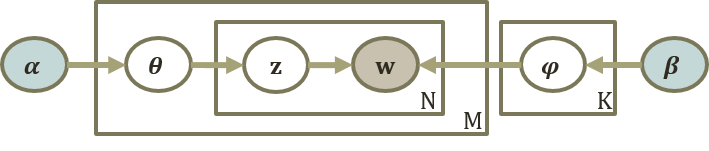
\includegraphics[scale=0.9]{fig10_21.png} 
\caption{토픽 모델링의 베이지안 네트워크 모델}
\label{fig:10-20}
\end{figure}

%슬라이드 27
이제 토픽 모델링에 적용할 수 있는 잠재 디리클레 할당(Latent Dirichlet Allocation, LDA)에 대해서 알아보도록 하겠다. 그러나 그 전에 토픽 모델링의 베이지안 네트워크가 어떻게 되는지를 먼저 자세히 알아보도록 하겠다. 그림 \ref{fig:10-20}의 그래프 모델은 토픽 모델링의 베이지안 네트워크를 나타낸다. $\alpha$와 $\beta$는 사전에 주어진 지식이며, $w$는 기사에 있는 개별 단어의 형태로 주어진 관찰 변수이다. 나머지는 모두 잠재 변수이다. 또한, 여기에는 베이지안 네트워크와 마찬가지로 chapter 7에서 다뤘던 판 표기법이 있으며, 이는 같은 불확실성 조건 하에서 생성되는 기사들과 기사 속 단어들을 그래프 모델로 나타내기 위해서 도입한 것이다. 그림 \ref{fig:10-20}에 따르면 여기에는 $M$개의 기사가 있으며 각 기사는 $\theta$라는 잠재 변수를 주제로 가진다. 또한, 각 기사에는 $N$개의 핵심 단어가 있으며, 이들 각각의 단어 또한 $z$라는 잠재 변수를 주제로 가진다. 토픽 모델링은 기사의 핵심 단어에 적절한 주제 $z$를 할당하는 것과 각 기사에 적절한 주제 $\theta$를 할당하는 과정을 포함한다. 여기서 우리는 $z$와 $w$가 각각 다항 분포로 되어 있다고 가정하겠다. 현실의 이슈, 그리고 그것과 관련된 단어는 원래부터 몇 개 내지는 수십 개에 불과하기 때문이다. \\

한편, 여기에는 $w$, $z$, $\theta$ 외에 사전 정보인 $\alpha$, $\beta$와 주제와 관련된 잠재 변수인 $\varphi$가 있다. 먼저 $\theta$는 $\alpha$를 파라미터로 가지는 디리클레 분포이다. 디리클레 분포(Dirichlet Distribution)란 다항 분포에 대한 켤레 사전 확률이 되는 확률 분포를 말하며, 다음과 같이 정의할 수 있다. 여기에는 먼저 2 이상의 자연수 $V$와 $V$차원 양수 벡터 $\alpha$가 있다. 그리고 디리클레 분포로부터 나타나는 $V$차원 확률 변수 $X$에 대해서는 모든 원소가 양의 실수이고, 그것들을 모두 합하면 정확히 1이 되어야 한다. 그러면 다음과 같이 확률 밀도 함수를 정의할 수 있다. 
\begin{equation}
P(X|\alpha) = \frac{\Gamma(\sum_{v=1}^{V} \alpha_{i})}{\prod_{v=1}^{V} \Gamma(\alpha_{v})} \prod_{v=1}^{V} x_{v}^{\alpha_{v}-1}
\label{eq:10-30-1}
\end{equation} 
수식 (\ref{eq:10-30-1})에서 $\Gamma(x)$는 감마 함수를 의미한다. 이러한 디리클레 분포는 베이즈 통계학에서 자주 쓰이는 확률 분포가 된다. 또한, 주제와 관련된 잠재 변수인 $\varphi$는 $z$와 함께 문서에 있는 단어 $w$를 결정한다. 여기서 $z$가 단어의 주제를 가리킨다면, $\varphi$는 주제별로 어떤 단어가 나타날지를 확률 정보로 나타낸다. 여기서 $\varphi$ 또한 숫자 $K$와 함께 판 표기법으로 표현되어 있으며, 이는 모두 $K$개의 주어가 있어서 각각의 주제는 서로 다른 확률 정보를 가진다는 것을 의미한다. 이렇게 $z$와 $\varphi$가 합쳐져서 $w$를 결정하는 형태가 되는 것이 바로 LDA 모델이 된다. $\varphi$는 $\theta$처럼 디리클레 분포를 따르며, 이것의 모수가 바로 $\beta$이다. 따라서 $\beta$는 이러한 $\varphi$에 대한 사전 정보가 된다. \\

\begin{figure}[ht] \centering 
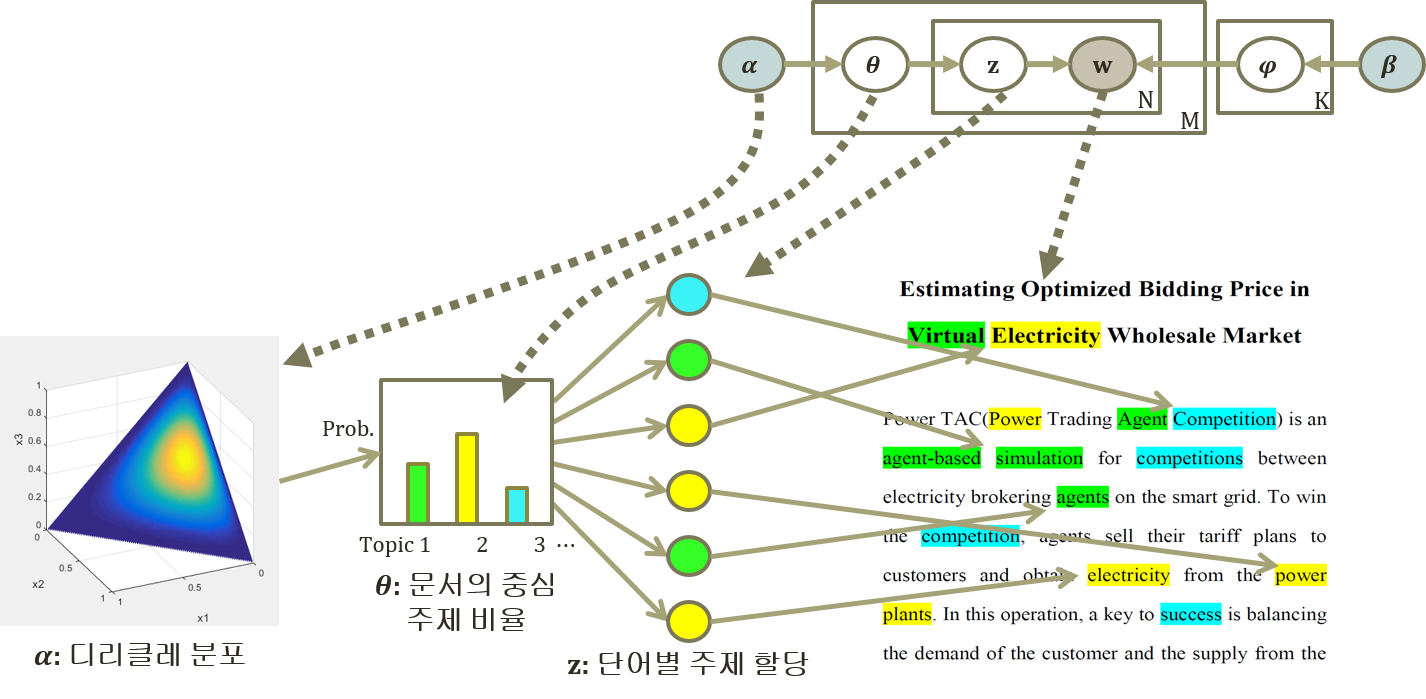
\includegraphics[scale=0.5]{fig10_20.png} 
\caption{실제 토픽 모델링 과정}
\label{fig:10-21}
\end{figure}

결국 LDA 모델이란 다음과 같다. 먼저 LDA 모델은 텍스트 데이터에 대한 약한 군집화이다. 또한 LDA 모델은 텍스트의 연속(Text Corpus)에 대한 구조를 베이지안 네트워크 형태로 표현한 것이다. 여기서는 판 표기법을 통해서 문서 내의 구조와 단어의 목록을 그래프 모형으로 나타내 주었다. 마지막으로 LDA 모델은 $\alpha$, $\beta$와 같은 사전 정보를 들고 있는 베이지안 네트워크 모델이 된다. 이러한 $\alpha$, $\beta$는 디리클레 분포가 가지는 파라미터 값이 되며, 각각 $\theta$와 $\varphi$를 생성하는데 있어서 영향을 준다. \\

%슬라이드 28
\begin{figure}[ht] \centering 
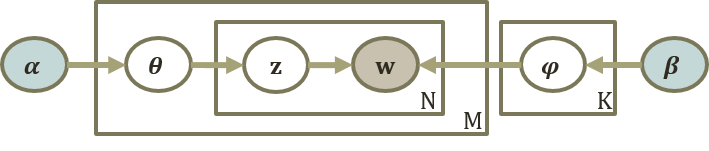
\includegraphics[scale=0.9]{fig10_21.png} 
\caption{토픽 모델링의 베이지안 네트워크 모델}
\label{fig:10-22}
\end{figure}

LDA 모델 또한 베이지안 네트워크 모델이므로 LDA 모델로부터 샘플을 생성하는 과정인 생성 과정(Generative Process)을 이해하고 있어야 한다. 여기서는 부모 노드가 없는 사전 정보인 $\alpha$에서부터 시작하겠다. $\alpha$는 디리클레 분포의 모수가 되는 사전 정보이며, 문서의 주제를 확률적으로 결정한다. 이것을 기준으로 해서 개별 문서의 주제를 할당한 것이 바로 $\theta_{i}$가 된다. 다음으로 $i$번째 문서에 있는 개별 단어의 주제 $z_{i,j}$는 $\theta_{i}$에서 나오는 확률값을 모수로 가지는 다항 분포로부터 생성된다. 한편, 또 다른 사전 정보인 $\beta$를 모수로 가지는 디리클레 분포로부터 $\varphi_{k}$, $k=1,\cdots,K$를 생성할 수 있다. 여기서 $\varphi_{k}$는 특정 단어가 $k$번째 주제를 가진다고 했을 때 단어의 표현이 어떤 식으로 나타나는지를 확률적으로 나타낸다. 그리고 이러한 $\varphi_{k}$에 단어의 주제를 나타내는 $z_{i,j}$를 결합한 $\varphi_{z_{i,j}}$를 모수로 가지는 다항 분포로부터 최종적으로 우리 눈에 보이는 단어인 $w_{i,j}$가 생성되는 것이다. 이것은 $i$번째 문서에 $j$번째 단어를 쓰기 위해서는 단어의 주제인 $z_{i,j}$를 생각하면서, 그 주제에 대해서 이야기하기 위해서 어떤 단어를 선택해야 할지를 나타내는 정보인 $\varphi_{z_{i,j}}$를 활용하겠다는 것이 된다. 이것을 바탕으로 우리에게 1,000개의 문서가 주어져 있고 한 개의 문서에 100개의 단어가 있다면 모두 100,000개의 단어가 위의 과정을 통해서 만들어졌다고 생각할 수 있다. \\ 

여기에서 가장 중요한 것은 개별 단어의 주제를 의미하는 $z$의 분포이다. 사전 정보인 $\alpha$, $\beta$와 관찰 변수인 $w$에 대해서는 이미 고정된 값이 주어져 있으므로 따로 값을 할당해야 하는 확률 변수로는 $\theta$, $\varphi$, 그리고 $z$가 있다. 그 중에서도 중간 지점에 위치한 $z$는 전체적인 추정에 있어서 중요한 역할을 한다. 만일 $z$의 값이 주어져 있다면 $z$와 $\alpha$ 사이의 $\theta$와 $z$, $w$와 $\beta$ 사이의 $\varphi$에 대해서 그 분포를 추정할 수 있게 된다. 여기서 $\theta$ 분포를 파악한다면 수많은 문서에서 전체적으로 어떤 주제가 많이 나타나는지를 알 수 있으며, $\varphi$ 분포를 파악한다면 특정 주제에서 어떤 어휘를 구사하는 것이 비율적으로 가장 적절한지를 확인할 수 있다. 다시 말해, $\theta$와 $\varphi$를 알 수 있다면 주어진 샘플로부터 현실의 정보를 캐낼 수 있는 것이다. 따라서 무엇보다도 $\theta$와 $\varphi$를 알아내는데 있어서 필수적인 $z$의 적절한 할당을 알아내는 것이야말로 이 문제의 핵심이 된다. \\         

%-----------------------------------------------------------------
\subsection{깁스 샘플링을 통한 주제 파악}
%-----------------------------------------------------------------

%슬라이드 29
이제 깁스 샘플링을 통해서 $z$에 가장 적절한 주제를 할당하는 방법에 대해서 알아야 한다. 기본적으로 깁스 샘플링은 베이지안 네트워크를 분석하는 방법이므로 이것의 결합 확률을 분해하는 것에서부터 시작을 해야 한다. 먼저 토픽 모델링의 베이지안 네트워크에서 결합 확률은 사전 정보인 $\alpha$, $\beta$, 관찰 변수인 $W$, 그리고 잠재 변수인 $z$, $\theta$, $\varphi$로 이루어져 있다. 따라서 이것의 결합 확률은 다음과 같은 형태로 주어진다.  
\begin{equation}
P(W,z,\theta,\varphi ; \alpha,\beta)
\label{eq:10-31}
\end{equation} 
여기서 특별히 쉼표 대신 세미콜론을 사용한 이유는 $\alpha$, $\beta$가 사전 정보라는 것을 분명히 밝히기 위해서이다. 분해 과정은 변수인 $W$, $z$, $\theta$, $\varphi$에 대해서 이루어진다. 먼저 $\varphi$의 경우에는 사전 정보인 $\beta$가 조건으로 주어져 있으며, 개별 사건 $k=1,\cdots,K$에 대해서 서로 독립인 $\varphi_k$끼리 확률식을 분해할 수 있다. 다음으로 $\theta$의 경우에는 사전 정보인 $\alpha$가 조건으로 주어져 있으며, 개별 문서 $i=1,\cdots,M$에 대해서 서로 독립인 $\theta_i$끼리 확률식을 분해할 수 있다. 마지막으로 $z$와 $W$의 경우에는 각각 $\theta_{i}$와 $\varphi_{z_{i,j}}$가 주어져 있으며, 문서 $i$의 개별 단어 $j=1,\cdots,N$에 대해서 각각 서로 독립인 $z_{i,j}$, $W_{i,j}$끼리 확률식을 분해할 수 있다. 지금까지의 설명을 실제 식으로 나타내면 다음과 같이 나온다. 
\begin{equation}
P(W,z,\theta,\varphi ; \alpha,\beta) = \prod_{k=1}^{K} P(\varphi_k:\beta) \prod_{i=1}^{M} P(\theta_i:\alpha) \prod_{j=1}^{N} P(z_{i,j}|\theta_i) P(W_{i,j}|\varphi_{z_{i,j}})   
\label{eq:10-32}
\end{equation} 
여기서 $P(\varphi_k:\beta)$는 $P(\varphi_k|\beta)P(\beta)$와, $P(\theta_i:\alpha)$는 $P(\theta_i|\alpha)P(\alpha)$와 같다. 이런 식으로 전체 결합 확률을 분해할 수 있는 것이다. \\

다음으로 변수를 중요한 변수와 덜 중요한 변수로 나누고, 결합 확률이 중요한 변수만을 다룰 수 있도록 하는 기법에 대해서 생각해 보도록 하겠다. 여기서는 일단 $\theta$와 $\varphi$를 다른 변수에 비해서 덜 중요하다고 판단할 수 있다. 왜냐하면 $W$는 관측 변수, $\alpha$, $\beta$는 사전 정보이므로 확률 계산에서 배재하기가 힘들며, 그 외에는 $z$를 일단 파악하고 있으면 나머지 $\theta$, $\varphi$에 대해서도 파악할 수 있기 때문이다. 직접적인 의미를 놓고 생각해 보아도 $z$는 단어에 대한 주제 할당을 뜻하므로 그 중요도가 높다는 것을 알 수 있다. 따라서 깁스 샘플링은 $z$ 변수를 대상으로 하며, 원활한 깁스 샘플링을 위해서 $\theta$와 $\varphi$를 없앨 필요가 있는 것이 된다. 이렇게 확률 계산에서 특정 변수를 없애고 난 후의 깁스 샘플링을 특별히 붕괴 깁스 샘플링(Collapsed Gibbs Sampling)이라고 부른다. \\

이와 같은 이유로 $\theta$와 $\varphi$를 제외하기로 결정했으므로 이제는 원래의 결합 확률에서 $\theta$와 $\varphi$를 없앨 방법에 대해서 생각해 보겠다. 이를 위한 가장 보편적인 방법으로 주변화가 있다. 다만 여기서는 $\theta$와 $\varphi$의 분포가 연속 확률 분포인 디리클레 분포이므로 개별 사건에 대해서 확률값을 합하는 대신에 모든 가능한 $\theta$, $\varphi$의 범위에 대해서 적분을 해야 한다. 따라서 우리가 해야 할 작업을 식으로 나타내면 다음과 같다.   
\begin{equation}
P(W,Z ; \alpha,\beta) = \int_{\theta} \int_{\varphi} P(W,z,\theta,\varphi ; \alpha,\beta) d\theta d\varphi
\label{eq:10-33}
\end{equation}
이것을 원래의 결합 확률을 생각해서 두 적분식의 곱으로 나타낼 수 있다. 먼저 $P(\varphi_k:\beta)$와 $P(W_{i,j}|\varphi_{z_{i,j}})$에는 $\theta$와는 관계 없이 $\varphi$만이 나와 있다. 따라서 이것들만을 따로 묶어서 $\varphi$에 대한 적분식으로 다음과 같이 나타낼 수 있다.     
\begin{equation}
\int_{\varphi} \prod_{k=1}^{K} P(\varphi_k:\beta) \prod_{i=1}^{M} \prod_{j=1}^{N} P(W_{i,j}|\varphi_{z_{i,j}}) d\varphi
\label{eq:10-34}
\end{equation} 
같은 식으로 $P(\theta_i:\alpha)$와 $P(z_{i,j}|\theta_i)$에는 $\varphi$와는 관계 없이 $\theta$만이 나와 있으므로, 이것들만을 따로 묶어서 $\theta$에 대한 적분식으로 다음과 같이 나타낼 수 있다. 
\begin{equation}
\int_{\theta} \prod_{i=1}^{M} P(\theta_i:\alpha) \prod_{j=1}^{N} P(z_{i,j}|\theta_i)  d\theta  
\label{eq:10-35}
\end{equation} 
이렇게 원래의 결합 확률을 수식 (\ref{eq:10-34})와 수식 (\ref{eq:10-35})의 곱으로 나타낼 수 있는 것이다. 그러나 여기서의 두 적분식 또한 매우 복잡한 형태이므로 이것을 통계학 기법으로 보다 단순하게 만들어 주어야 한다. \\

%슬라이드 30
먼저 수식 (\ref{eq:10-34})을 어떻게 나타낼 것인지에 대해서 생각해 보겠다. 이를 위해서는 먼저 구체적인 $\varphi$의 형태를 생각해 보아야 한다. $\varphi$는 행렬의 형태로 나타나며, 각각의 행은 하나의 주제를, 열은 하나의 단어를 의미한다. 그리고 마치 사전과 같이 우리에게 단어 리스트가 주어졌다고 하면, $\varphi_{k,v}$의 값은 $k$번째에 해당되는 주제를 가지는 단어가 단어 리스트의 $v$번째 단어일 확률이 된다. 예를 들어, $\varphi$의 열일곱 번째 열이 의미하는 단어가 카이스트라면 각 행의 열일곱 번째 값은 특정 주제를 생각하면서 사용한 단어가 카이스트와 일치할 확률을 의미하게 된다. 이러한 정의에 따르면 $\varphi$ 행렬에서 같은 행에 있는 모든 원소를 합하면 정확히 $1$이라는 값이 나온다. 그리고 각각의 주제는 모두 독립이므로 $\varphi$를 행별로 분리한 $\varphi_k$ 또한 서로 독립이다. 따라서 원래의 수식 (\ref{eq:10-34})를 다음과 같이 각각의 $k$에 대해서 서로 다른 적분 계산을 해서 곱하는 형태의 식으로 바꿀 수 있다. 
\begin{equation}
\prod_{k=1}^{K} \int_{\varphi_{k}} P(\varphi_{k}:\beta) \prod_{i=1}^{M} \prod_{j=1}^{N} P(W_{i,j}|\varphi_{z_{i,j}}) d\varphi_{k}
\label{eq:10-36}
\end{equation} 
이제 수식 (\ref{eq:10-30-1})에서 제시한 디리클레 분포의 확률 밀도 함수를 $P(\varphi_{k}:\beta)$에 대입해 주자. 그러면 다음과 같은 수식을 얻을 수 있다.
\begin{equation}
\prod_{k=1}^{K} \int_{\varphi_{k}} \frac{\Gamma(\sum_{v=1}^{V} \beta_{i})}{\prod_{v=1}^{V} \Gamma(\beta_{v})} \prod_{v=1}^{V} \varphi_{k,v}^{\beta_{v}-1} \prod_{i=1}^{M} \prod_{j=1}^{N} P(W_{i,j}|\varphi_{z_{i,j}}) d\varphi_{k}
\label{eq:10-37}
\end{equation} \\

다음으로 $P(W_{i,j}|\varphi_{z_{i,j}})$에 다항 분포의 확률 분포 함수를 대입해 주어야 한다. 여기서는 일단 각 $i$, $j$에 대해서 이러한 함수가 있으며, 최종 확률을 구하기 위해서는 이들을 모두 곱해야 한다는 것을 생각해서 식을 더욱 간단하게 표현할 수 있다. 먼저 $i$번째 문서에서 $k$번째 주제를 가지는 단어 중에서 단어 리스트의 $v$번째 단어가 몇 번이나 등장하는지를 정수 $n_{i,v}^{k}$로 나타내도록 하겠다. 예를 들어, 우리에게 $M=10$개의 문서와 $V=50$개의 단어를 가진 단어 리스트가 주어졌으며, 생각할 수 있는 주제는 $K=2$가지가 있다고 하겠다. 우리는 7번째 문서에서 단어 리스트의 17번째 단어인 카이스트가 주제별로 얼마나 자주 등장하는지를 알아야 한다고 가정하겠다. 그러면 우리는 먼저 7번째 문서의 단어를 각 주제별로 분류하고, 각각의 분류에 대해서 카이스트가 얼마나 자주 등장하는지를 헤아리면 된다. 여기서는 첫 번째 주제에 대해서 2번, 두 번째 주제에 대해서 1번 나왔다고 가정하겠다. 그러면 $i=7$, $v=17$이므로 $n_{7,17}^{1}$은 2, $n_{7,17}^{2}$는 1이 된다. 우리는 이러한 작업을 각각의 문서에 대해서, 각각의 주제에 대해서, 그리고 각각의 단어에 대해서 시행할 수 있다. 또한, 여기서는 특별히 모든 문서들을 하나로 놓고 이러한 작업을 시행한 결과값을 $n_{(.),v}^{k}$라고 정하였으며, 이것은 각 $i$에 대해서 $n_{i,v}^{k}$를 모두 합친 것과 같다. \\

이제 원래의 식으로 돌아가서, 우리의 목적이었던 $P(W_{i,j}|\varphi_{z_{i,j}})$의 수식 표현에 대해서 다시 생각해 보자. $i$번째 문서의 $j$번째 단어가 $k$번째 주제에 속하면서 단어 리스트의 $v$번째 단어와 같다면 $P(W_{i,j}|\varphi_{z_{i,j}})$는 다항 분포의 정의에 의해서 앞에서의 설명에 해당되는 확률값인 $\varphi_{k,v}$와 같게 된다. 그리고 수식 (\ref{eq:10-37})에서는 이러한 $P(W_{i,j}|\varphi_{z_{i,j}})$를 모든 문서 $i=1,\cdots,m$의 모든 단어 $j=1,\cdots,n$에 대해서 곱하고 있다. 그러면 원래의 식에서$\varphi_{k,v}$가 곱해지는 횟수는, 모든 문서의 $k$번째 주제에 속하는 단어들 중에서 단어 리스트의 $v$번째 단어가 나오는 개수만큼이 된다. 따라서 앞서 정의한 $n_{(.),v}^{k}$를 사용해서 전체 $\prod_{i=1}^{M} \prod_{j=1}^{N} P(W_{i,j}|\varphi_{z_{i,j}})$와 같은 형태의 식을 $\prod_{v=1}^{V} \varphi_{k,v}^{n_{(.),v}^{k}}$처럼 바꿔서 표현할 수 있게 된다. 그리고 이를 반영해서 수식 (\ref{eq:10-37})을 다음과 같이 전개해 나갈 수 있다. 
\begin{equation}
\prod_{k=1}^{K} \int_{\varphi_{k}} \frac{\Gamma(\sum_{v=1}^{V} \beta_{v})}{\prod_{v=1}^{V} \Gamma(\beta_{v})} \cdot \prod_{v=1}^{V} \varphi_{k,v}^{\beta_{v}-1} \cdot \prod_{v=1}^{V} \varphi_{k,v}^{n_{(.),v}^{k}} d\varphi_{k}
\label{eq:10-38}
\end{equation}
그리고 이것을 같은 $\varphi_{k,v}$끼리 묶어서 곱해주고, $\varphi_{k}$와 관련 없는 상수를 적분 밖으로 이동시키면 다음과 같이 새로운 형태의 식을 유도할 수 있다. 
\begin{equation}
\prod_{k=1}^{K} \frac{\Gamma(\sum_{v=1}^{V} \beta_{v})}{\prod_{v=1}^{V} \Gamma(\beta_{v})} \int_{\varphi_{k}} \prod_{v=1}^{V} \varphi_{k,v}^{n_{(.),v}^{k}+\beta_{v}-1} d\varphi_{k}
\label{eq:10-39}
\end{equation} 

그러면 우리에게는 수식에 통계학 기법을 적용해서 더욱 단순한 형태의 수식으로 나타내는 마지막 과정이 남아 있게 된다. 이를 진행하기 위해서는 먼저 $\varphi_{k,v}$를 $n_{(.),v}^{k}+\beta_{v}-1$번 곱하는 것과 디리클레 분포의 확률 밀도 함수에서 $x_{v}$를 $\alpha_{v}$번 곱하는 것의 형태가 서로 비슷하다는 것을 이용해서, 수식 (\ref{eq:10-39})의 $\varphi_{k,v}$에 관한 항을 파라미터 $n_{(.),v}^{k}+\beta_{v}$를 가지는 디리클레 분포의 확률 밀도 함수로 나타내 주어야 한다. 우리는 이를 디리클레 분포의 확률 밀도 함수를 구성하기 위해서 필요한 상수를 적분식 안에서는 곱해주고, 곱해진 수를 상쇄하기 위한 목적으로 적분식 밖에서는 나눠주는 식으로 수행할 수 있다. 
\begin{equation}
\prod_{k=1}^{K} \frac{\Gamma(\sum_{v=1}^{V} \beta_{v})}{\prod_{v=1}^{V} \Gamma(\beta_{v})} \frac{\prod_{v=1}^{V} \Gamma(n_{(.),v}^{k}+\beta_{v})}{\Gamma(\sum_{v=1}^{V} n_{(.),v}^{k}+\beta_{v})} \int_{\varphi_{k}}    P(\varphi_{k}|n_{(.),v}^{k}+\beta_{v}) d\varphi_{k}
\label{eq:10-40}
\end{equation}
여기서 $P(\varphi_{k}|n_{(.),v}^{k}+\beta_{v})$는 파라미터 $n_{(.),v}^{k}+\beta_{v}$를 가지는 디리클레 분포의 확률 밀도 함수를 의미한다. 그러면 확률 밀도 함수를 $\varphi_{k}$의 전 범위에 대해서 적분한 식은 정확히 $1$이 되므로 이를 반영하고 식의 형태를 정리하면 다음과 같이 우리가 원하는 수식 (\ref{eq:10-34})의 최종 전개 결과가 나오게 된다.
\begin{equation}
\prod_{k=1}^{K} \frac{\prod_{v=1}^{V} \Gamma(n_{(.),v}^{k}+\beta_{v}) \cdot \Gamma(\sum_{v=1}^{V} \beta_{v})}{\prod_{v=1}^{V} \Gamma(\beta_{v}) \cdot \Gamma(\sum_{v=1}^{V} n_{(.),v}^{k}+\beta_{v})}
\label{eq:10-41}
\end{equation}
이것으로 결합 확률을 이루는 부분 중 하나인 수식 (\ref{eq:10-34})을 적분 없이 나타낼 수 있다. \\

%슬라이드 32
한편, 이런 식으로 적분식을 제거할 수 있었던 이유는 다항 분포의 확률 분포 함수와 디리클레 분포의 확률 밀도 함수를 곱한 식으로부터 또 다른 디리클레 분포의 확률 밀도 함수를 유도하였기 때문이다. LDA에서는 이들 분포 함수의 곱을 다음과 같은 형태로 나타낼 수 있다.    
\begin{equation}
\int_{\theta} \prod_{i=1}^{M} P(\theta_{i} ; \alpha) \prod_{j=1}^{N} P(z_{i,j}|\theta_{i}) d\theta
\label{eq:10-41-1}
\end{equation}
이것의 일반적인 형태로는 사전 지식에 관한 확률인 $P(\theta)$와 조건부 확률인 $P(Z|\theta)$, 이렇게 두 개의 확률의 곱이 된다. 이 때, $P(\theta)$와 $P(Z|\theta)$의 곱으로부터 상수를 곱하는 등의 다소의 전개 과정을 거쳐서 다시 사전 지식에 관한 확률 $P(\theta')$을 유도해 낼 수 있다면 이들 두 확률을 켤레 사전 확률(Conjugate Prior)이라고 부른다. 그러면 이제는 확률 밀도 함수를 모든 사건에 대해서 적분하면 1이 된다는 통계학 지식을 활용해서, 앞에서 했던 것처럼 켤레 사전관계 사이인 두 확률 함수의 곱이 들어간 적분식을 소거해줄 수 있게 된다.      디리클레 분포와 다항 분포는 대표적인 켤레 사전 확률이며, 우리는 이것을 붕괴 깁스 샘플링을 위한 결합 확률의 계산에 활용하였다. \\
 
%슬라이드 31
수식 (\ref{eq:10-35}) 또한 비슷한 형태의 수식 (\ref{eq:10-34})에서 그랬던 것처럼 유사한 과정을 통해서 적분을 제외한 식으로 나타낼 수 있다. 먼저 개별 텍스트는 독립이므로 서로 다른 $\theta_{i}$ 또한 독립적으로 적용된다. 따라서 우리는 수식 (\ref{eq:10-35})의 적분을 개별 $\theta_{i}$에 대한 적분의 곱으로 다음과 같이 나타낼 수 있다.
\begin{equation}
\prod_{i=1}^{M} \int_{\theta_{i}} P(\theta_i:\alpha) \prod_{j=1}^{N} P(z_{i,j}|\theta_i) d\theta_{i} 
\label{eq:10-43}
\end{equation}
다음으로 디리클레 분포의 확률 밀도 함수를 $P(\theta_i:\alpha)$에 대입하여 다음과 같이 나타내어 줄 수 있다.  
\begin{equation}
\prod_{i=1}^{M} \int_{\theta_{i}} \frac{\Gamma(\sum_{k=1}^{K} \alpha_{k})}{\prod_{k=1}^{K} \Gamma(\alpha_{k})}  \prod_{k=1}^{K} \theta_{i,k}^{\alpha_{k}-1} \prod_{j=1}^{N} P(z_{i,j}|\theta_i) d\theta_{i} 
\label{eq:10-44}
\end{equation}
다음으로 다항 분포의 확률 분포 함수를 각 단어 $j$에 대해서 곱한 $\prod_{j=1}^{N} P(z_{i,j}|\theta_i)$를 새롭게 나타내어 보자. 앞에서처럼 $P(z_{i,j}|\theta_i)$는 $i$번째 문서의 $j$번째 단어가 $k$번째 주제에 속할 확률을 나타내므로 다항 분포의 정의에 의해서 $\theta_{i,k}$와 그 값이 같게 나온다. 수식 (\ref{eq:10-35})에서는 각 단어 $j$에 대해서 그에 해당하는 확률값인 $\theta_{i,k}$를 계속 곱하고 있다. 따라서 이것은 특정 문서에서 $k$번째 주제를 가진 단어가 몇 개나 되는지를 헤아려서 그 횟수만큼 $\theta_{i,k}$를 곱하는 것과 같다. 여기서는 이것을 $n_{i,(.)}^{k}$라고 정하였으며, 앞에서 정의한 $n_{i,v}^{k}$를 사용해서 설명한다면 이것은 각 $v$에 대해서 $n_{i,v}^{k}$를 모두 합친 것과 같다. 우리는 $n_{i,(.)}^{k}$를 활용해서 원래의 수식을 다음과 같이 나타낼 수 있다.    
\begin{equation}
\prod_{i=1}^{M}  \int_{\theta_{i}} \frac{\Gamma(\sum_{k=1}^{K} \alpha_{k})}{\prod_{k=1}^{K} \Gamma(\alpha_{k})}  \prod_{k=1}^{K} \theta_{i,k}^{\alpha_{k}-1} \cdot \prod_{k=1}^{K} \theta_{i,k}^{n^{k}_{i,(.)}} d\theta_{i} 
\label{eq:10-45}
\end{equation}
그리고 이것을 같은 $\theta_{i,k}$끼리 묶어서 곱해주고, $\theta_{i,k}$와 관련 없는 상수를 적분 밖으로 이동시키면 다음과 같은 식을 구할 수 있다.
\begin{equation}
\prod_{i=1}^{M} \frac{\Gamma(\sum_{k=1}^{K} \alpha_{k})}{\prod_{k=1}^{K} \Gamma(\alpha_{k})} \int_{\theta_{i}} \prod_{k=1}^{K} \theta_{i,k}^{n^{k}_{i,(.)}+\alpha_{k}-1} d\theta_{i} 
\label{eq:10-46}
\end{equation}
이제 남은 것은 위에서와 마찬가지로 통계학 기법을 활용해서 적분 안의 $\prod_{k=1}^{K} \theta_{i,k}^{n^{k}_{i,(.)}+\alpha_{k}-1}$를 디리클레 분포의 확률 밀도 함수로 바꾸는 것이 된다. 여기서는 파라미터로 $n^{k}_{i,(.)}+\alpha_{k}$를 가지는 디리클레 분포를 구성하기 위해서 필요한 상수를 적분식 안에서는 곱해주고, 적분식 밖에서는 나눠준다. 그러면 새로운 디리클레 분포의 확률 밀도 함수인 $P(\theta_{i}|n^{k}_{i,(.)}+\alpha_{k})$가 홀로 적분식 안에 있는 수식을 다음과 같이 나타낼 수 있다. 
\begin{equation}
\prod_{i=1}^{M} \frac{\Gamma(\sum_{k=1}^{K} \alpha_{k})}{\prod_{k=1}^{K} \Gamma(\alpha_{k})} \frac{\prod_{k=1}^{K} \Gamma(n^{k}_{i,(.)}+\alpha_{k})}{\Gamma(\sum_{k=1}^{K} n^{k}_{i,(.)}+\alpha_{k})} \int_{\theta_{i}} P(\theta_{i}|n^{k}_{i,(.)}+\alpha_{k})  d\theta_{i} 
\label{eq:10-47}
\end{equation}
그러면 확률 밀도 함수의 정의에 따라서 적분식의 값은 정확히 1이 되므로 우리는 적분식을 원래의 식으로부터 제외할 수 있다. 그리고 이것을 정리해서 원래의 수식 (\ref{eq:10-35})를 다음과 같이 적분식이 없는 수식으로 나타낼 수 있다.  
\begin{equation}
\prod_{i=1}^{M} \frac{\prod_{k=1}^{K} \Gamma(n^{k}_{i,(.)}+\alpha_{k}) \cdot \Gamma(\sum_{k=1}^{K} \alpha_{k})}{\prod_{k=1}^{K} \Gamma(\alpha_{k}) \cdot \Gamma(\sum_{k=1}^{K} n^{k}_{i,(.)}+\alpha_{k})}
\label{eq:10-48}
\end{equation}

결국 우리가 처음에 구하고자 한 확률인 $P(W,Z ; \alpha,\beta)$은 다음과 같이 수식 (\ref{eq:10-41})과 수식 (\ref{eq:10-48})의 곱으로 나타내어진다. \\
\begin{equation}
P(W,Z ; \alpha,\beta) = \prod_{k=1}^{K} \frac{\prod_{v=1}^{V} \Gamma(n_{(.),v}^{k}+\beta_{v}) \cdot \Gamma(\sum_{v=1}^{V} \beta_{v})}{\prod_{v=1}^{V} \Gamma(\beta_{v}) \cdot \Gamma(\sum_{v=1}^{V} n_{(.),v}^{k}+\beta_{v})} \cdot \prod_{i=1}^{M} \frac{\prod_{k=1}^{K} \Gamma(n^{k}_{i,(.)}+\alpha_{k}) \cdot \Gamma(\sum_{k=1}^{K} \alpha_{k})}{\prod_{k=1}^{K} \Gamma(\alpha_{k}) \cdot \Gamma(\sum_{k=1}^{K} n^{k}_{i,(.)}+\alpha_{k})}
\label{eq:10-49}
\end{equation}

%-----------------------------------------------------------------
\subsection{깁스 샘플링 공식}
%-----------------------------------------------------------------
%슬라이드 33
앞서 우리는 전체적인 결합 확률이 주어진 상황에서 $\theta$와 $\varphi$를 주변화한 확률인 $P(W,Z ; \alpha,\beta)$을 어떻게 구성할 지에 대해서 생각하였다. 여기서 $W$는 관찰 변수, $\alpha$, $\beta$는 사전 지식에 해당하므로, 이제 우리의 목표는 적절한 $Z$의 할당을 찾는 것이 된다. 앞서 설명한 깁스 샘플링은 특정 시점에서의 $Z$값이 주어졌을 때, 시간의 흐름에 따라 $Z$의 원소들을 하나씩 갱신하는 작업을 진행한다. 다음의 그림은 깁스 샘플링의 과정을 잘 보여준다. \\
    
\begin{figure}[ht] \centering 
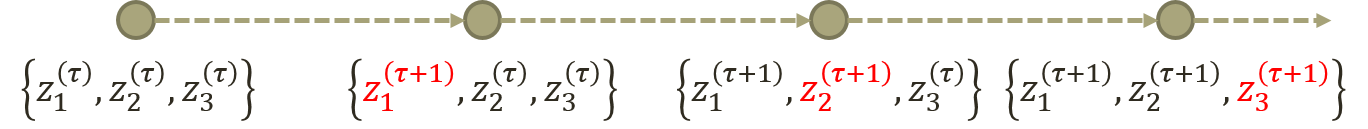
\includegraphics[scale=0.5]{fig10_13.png} 
\caption{세 잠재 변수에서의 깁스 샘플링 과정}
\label{fig:10-23}
\end{figure}

LDA에서 깁스 샘플링을 실행하기 위해서는 다른 모든 단어의 주제가 고정된 상황에서 특정 $i$번째 문서의 $j$번째 단어의 주제에 대한 적절한 샘플링이 이루어져야 한다. 따라서 $i$번째 문서의 $j$번째 단어에 적절한 주제를 새로 할당할 수 있도록 하는 수식을 세워야 한다. 여기서는 $i$번째 문서의 $j$번째 단어에 할당된 주제를 $Z_{(i,j)}$, 그 외 단어에 주어져 있는 주제를 $Z_{-(i,j)}$라고 하겠다. 그러면 관찰 변수 $W$와 사전 지식 $\alpha$, $\beta$, 그리고 $Z_{(i,j)}$ 외의 모든 잠재 변수가 주어진 상황에서, $Z_{(i,j)}$에 $l$번째 주제가 할당되었을 확률을 다음과 같이 세울 수 있다.
\begin{equation}
P(Z_{(i,j)} = l|Z_{-(i,j)}, W ; \alpha,\beta) = \frac{P(Z_{(i,j)} = l, Z_{-(i,j)}, W ; \alpha,\beta)}{P(Z_{-(i,j)}, W ; \alpha,\beta)}
\label{eq:10-50}
\end{equation}
여기서 $P(Z_{-(i,j)}, W ; \alpha,\beta)$는 주어진 정보에 대한 결합 확률이므로 상수에 불과하게 된다. 따라서 수식 (\ref{eq:10-50})의 조건부 확률은 다음의 결합 확률과 정비례하게 된다.
\begin{equation}
P(Z_{(i,j)} = l|Z_{-(i,j)}, W ; \alpha,\beta) \propto P(Z_{(i,j)} = l, Z_{-(i,j)}, W ; \alpha,\beta)
\label{eq:10-51}
\end{equation} 
따라서 우리는 여기서 나온 결합 확률을 어떻게 계산할지를 생각하면 된다. \\

%슬라이드 34
수식 (\ref{eq:10-51})의 샘플링을 위한 결합 확률을 계산하기 위해서, 앞에서 구한 일반적인 결합 확률인 $P(W,Z ; \alpha,\beta)$를 보다 더 간단히 나타내는 전개 과정에 대해서 먼저 생각해보도록 하겠다. 우리는 앞에서 이미 $P(W,Z ; \alpha,\beta)$의 확률값을 다음 두 식의 곱으로 나타내 주었다.
\begin{equation}
\prod_{k=1}^{K} \frac{\prod_{v=1}^{V} \Gamma(n_{(.),v}^{k}+\beta_{v}) \cdot \Gamma(\sum_{v=1}^{V} \beta_{v})}{\prod_{v=1}^{V} \Gamma(\beta_{v}) \cdot \Gamma(\sum_{v=1}^{V} n_{(.),v}^{k}+\beta_{v})} \cdot \prod_{i=1}^{M} \frac{\prod_{k=1}^{K} \Gamma(n^{k}_{i,(.)}+\alpha_{k}) \cdot \Gamma(\sum_{k=1}^{K} \alpha_{k})}{\prod_{k=1}^{K} \Gamma(\alpha_{k}) \cdot \Gamma(\sum_{k=1}^{K} n^{k}_{i,(.)}+\alpha_{k})}
\label{eq:10-52}
\end{equation}
여기서 첫 번째 식에서 $k$와 관련 없는 항과 두 번째 식에서 $i$와 관련 없는 항을 각각 $K$번, $M$번씩 곱해서 앞으로 빼내면 다음과 같은 식을 얻을 수 있다.  
\begin{equation}
(\frac{\Gamma(\sum_{v=1}^{V} \beta_{v})}{\prod_{v=1}^{V} \Gamma(\beta_{v})})^{K} (\frac{\Gamma(\sum_{k=1}^{K} \alpha_{k})}{\prod_{k=1}^{K} \Gamma(\alpha_{k})})^{M} \prod_{k=1}^{K} \frac{\prod_{v=1}^{V} \Gamma(n_{(.),v}^{k}+\beta_{v})}{\Gamma(\sum_{v=1}^{V} n_{(.),v}^{k}+\beta_{v})} \prod_{i=1}^{M} \frac{\prod_{k=1}^{K} \Gamma(n^{k}_{i,(.)}+\alpha_{k})}{\Gamma(\sum_{k=1}^{K} n^{k}_{i,(.)}+\alpha_{k})}
\label{eq:10-53}
\end{equation}
이렇게 앞으로 빼낸 식은 사전 확률인 $\alpha$, $\beta$로만 나타내어지며, 샘플링에 의해서 결정되는 $n^{k}_{i,(.)}$, $n^{k}_{(.),v}$와는 독립이므로 샘플링을 위한 결합 확률의 계산에 있어서는 이것을 상수로 간주할 수 있다. 따라서 우리는 원래의 $P(W,Z ; \alpha,\beta)$와 정비례하는 다음 식의 값만을 고려하면 된다.
\begin{equation}
\prod_{k=1}^{K} \frac{\prod_{v=1}^{V} \Gamma(n_{(.),v}^{k}+\beta_{v})}{\Gamma(\sum_{v=1}^{V} n_{(.),v}^{k}+\beta_{v})} \cdot \prod_{i=1}^{M} \frac{\prod_{k=1}^{K} \Gamma(n^{k}_{i,(.)}+\alpha_{k})}{\Gamma(\sum_{k=1}^{K} n^{k}_{i,(.)}+\alpha_{k})}
\label{eq:10-54}
\end{equation}

이제 우리가 원하는 수식 (\ref{eq:10-51})의 결합 확률을 구하기 위해서는 $i$번째 문서, $j$번째 단어의 주제가 되는 잠재 변수 $Z_{(i,j)}$가 $l$번째 주제에 해당되는 경우만을 생각하면 된다. 그 외의 문서, 단어에 관련된 확률값은 상수로 간주되어 더 이상 생각할 필요가 없다. 먼저 두 번째 식에는 여러 개의 문서를 다룬다는 의미로 모든 문서에 대한 확률값이 곱해져 있다. 그러나 이제는 특정 $i$번째 문서에만 관심이 있으므로 $i$번째 문서 외의 나머지 문서와 관련된 확률값을 상수로 생각할 수 있다. 따라서 우리가 감안해야 할 확률값을 다음과 같이 축소할 수 있다.    
\begin{equation}
\prod_{k=1}^{K} \frac{\prod_{v=1}^{V} \Gamma(n_{(.),v}^{k}+\beta_{v})}{\Gamma(\sum_{v=1}^{V} n_{(.),v}^{k}+\beta_{v})} \cdot \frac{\prod_{k=1}^{K} \Gamma(n^{k}_{i,(.)}+\alpha_{k})}{\Gamma(\sum_{k=1}^{K} n^{k}_{i,(.)}+\alpha_{k})}
\label{eq:10-55}
\end{equation}

다음으로는 우리가 $j$번째 단어에만 관심이 있다는 사실을 반영해 주도록 하겠다. 먼저 $i$번째 문서의 $j$번째 단어가 우리에게 주어진 단어 리스트의 $v^{*}$번째 단어에 해당된다고 가정하자. 그러면 우리는 $v^{*}$ 외의 다른 단어를 신경 쓸 필요가 없다. 따라서 첫 번째 식에서 $\Gamma(n_{(.),v}^{k}+\beta_{v})$를 각 $v$에 대해서 모두 곱한 것은 $v=v^{*}$인 경우 외의 다른 $v$에 대한 값을 더 이상 고려하지 않아도 된다. 따라서 원래의 식을 다음과 같은 형태로 또 다시 축소할 수 있다. 
\begin{equation}
\prod_{k=1}^{K} \frac{\Gamma(n_{(.),v^{*}}^{k}+\beta_{v^{*}})}{\Gamma(\sum_{v=1}^{V} n_{(.),v}^{k}+\beta_{v})} \cdot \frac{\prod_{k=1}^{K} \Gamma(n^{k}_{i,(.)}+\alpha_{k})}{\Gamma(\sum_{k=1}^{K} n^{k}_{i,(.)}+\alpha_{k})}
\label{eq:10-56}
\end{equation}

마지막으로 두 번째 식의 분모인 $\Gamma(\sum_{k=1}^{K} n^{k}_{i,(.)}+\alpha_{k})$의 경우에는 잠재 변수 $Z_{(i,j)}$의 할당을 바꿔주더라도 $n^{k}_{i,(.)}$을 모든 $k$에 대해서 합해준 값은 변하지 않으므로 마찬가지로 상수로 생각해 줄 수 있다. 따라서 우리가 최종적으로 고려해야 할 식은 다음과 같은 형태로 나타난다. 
\begin{equation}
\prod_{k=1}^{K} \frac{\Gamma(n_{(.),v}^{k}+\beta_{v})}{\Gamma(\sum_{v=1}^{V} n_{(.),v}^{k}+\beta_{v})} \cdot \prod_{k=1}^{K} \Gamma(n^{k}_{i,(.)}+\alpha_{k})
\label{eq:10-57}
\end{equation}
이러한 수식 (\ref{eq:10-57})은 수식 (\ref{eq:10-51})의 결합 확률에 정비례한다. \\

%슬라이드 35
이제는 잠재 변수 $Z_{(i,j)}$가 $l$이라는 것을 본격적으로 반영해서 식을 전개해 나갈 것이며, 이를 위해서는 또다시 새로운 개념의 정의가 필요하다. 앞에서 우리는 $i$번째 문서에서 $k$번째 주제를 가지는 단어들 중 단어 리스트의 $v$번째 단어가 등장하는 횟수를 $n_{i,v}^{k}$로 정의하였다. 새로운 개념은 $i$번째 문서의 $j$번째 단어를 제외한 나머지에 대해서 해당 단어가 나오는 횟수로 정의할 수 있으며, 이것을 $n_{i,v}^{k,-(i,j)}$로 나타내도록 하겠다. 이러한 개념을 따로 정의하는 이유는 바로 $Z_{(i,j)} = l$에 따라서 $i$번째 문서의 $j$번째 단어가 $l$번째 주제를 가진다는 것을 수식에 반영하기 위해서이다. 한편, 앞에서와 마찬가지로 $n_{(.),v}^{k,-(i,j)}$는 $i$번째 문서의 $j$번째 단어를 제외한 나머지 모든 문서의 단어에서 단어 리스트의 $v$번째 단어가 나오는 횟수를 말한다. 그리고 $n_{i,(.)}^{k,-(i,j)}$는 단어의 형태와는 상관 없이 $i$번째 문서의 $j$번째 단어를 제외한 나머지 단어들이 $k$번째 주제를 가지게 되는 횟수를 말한다. \\

수식 (\ref{eq:10-57})은 주어진 식들을 $k=1$에서 $k=K$까지 곱하는 형태로 되어 있다. 이제는 이것을 $k \neq l$인 경우와 $k=l$인 경우로 분리하면서 $k=l$인 경우에 대해서는 $l$번째 주제를 가지는 단어가 하나 추가되었음을 식에 분명히 나타낼 필요가 있다. 먼저 $k \neq l$인 경우의 식은 $n_{(.),v}^{k}$와 $n_{i,v}^{k,-(i,j)}$가 같으므로, $n_{i,v}^{k,-(i,j)}$를 $n_{(.),v}^{k}$가 있던 자리에 그대로 대입해서 다음과 같이 나타낼 수 있다. 
\begin{equation}
\prod_{k=1, k \neq l}^{K} \frac{\Gamma(n_{(.),v}^{k,-(i,j)}+\beta_{v})}{\Gamma(\sum_{v=1}^{V} n_{(.),v}^{k,-(i,j)}+\beta_{v})} \cdot \prod_{k=1, k \neq l}^{K} \Gamma(n^{k,-(i,j)}_{i,(.)}+\alpha_{k})
\label{eq:10-58}
\end{equation}
그리고 $k=l$인 경우의 식은 $l$번째 주제의 단어가 하나 더해졌기 때문에, $n_{(.),v}^{l,-(i,j)}$에 $1$을 추가해서 다음과 같이 나타낼 수 있다.
\begin{equation}
\frac{\Gamma(n_{(.),v}^{l,-(i,j)}+\beta_{v}+1)}{\Gamma(\sum_{v=1}^{V} n_{(.),v}^{l,-(i,j)}+\beta_{v}+1)} \cdot \Gamma(n^{l,-(i,j)}_{i,(.)}+\alpha_{l}+1)
\label{eq:10-59}
\end{equation} 
여기에 감마 함수의 기본 성질 중 하나인 $\Gamma(y+1)$와 $y \cdot \Gamma(y)$가 같은 값을 가진다는 성질을 활용해서, 감마 함수 안의 $1$을 차례대로 정리하면 다음과 같은 식으로 나타낼 수 있다.
\begin{equation}
\frac{\Gamma(n_{(.),v}^{l,-(i,j)}+\beta_{v})}{\Gamma(\sum_{v=1}^{V} n_{(.),v}^{l,-(i,j)}+\beta_{v})} \cdot \Gamma(n^{l,-(i,j)}_{i,(.)}+\alpha_{l}) \cdot \frac{n_{(.),v}^{l,-(i,j)}+\beta_{v}}{\sum_{v=1}^{V} n_{(.),v}^{l,-(i,j)}+\beta_{v}} \cdot (n^{l,-(i,j)}_{i,(.)}+\alpha_{l})
\label{eq:10-60}
\end{equation} 

%슬라이드 36
여기서 수식 (\ref{eq:10-57})은 수식 (\ref{eq:10-58})과 수식 (\ref{eq:10-60})의 곱으로 되어 있다. 따라서 수식 (\ref{eq:10-58})에서 각 $k$에 대한 식들을 곱할 때 $k=l$일 때의 식은 제외하고 곱했던 것을, 수식 (\ref{eq:10-60})으로부터 $k=l$일 때의 식을 다시 가져와서 보충할 수 있게 된다. 그러면 수식 (\ref{eq:10-58})은 다음과 같이 모든 $k$에 대한 식들을 곱한 형태로 나타낼 수 있다.
\begin{equation}
\prod_{k=1}^{K} \frac{\Gamma(n_{(.),v}^{k,-(i,j)}+\beta_{v})}{\Gamma(\sum_{v=1}^{V} n_{(.),v}^{k,-(i,j)}+\beta_{v})} \cdot \prod_{k=1}^{K} \Gamma(n^{k,-(i,j)}_{i,(.)}+\alpha_{k})
\label{eq:10-61}
\end{equation}
그리고 수식 (\ref{eq:10-60})은 수식 (\ref{eq:10-58})에 보태진 식이 그대로 빠져나가면서 다음과 같은 형태로 나타내어진다.
\begin{equation}
\frac{n_{(.),v}^{l,-(i,j)}+\beta_{v}}{\sum_{v=1}^{V} n_{(.),v}^{l,-(i,j)}+\beta_{v}} \cdot (n^{l,-(i,j)}_{i,(.)}+\alpha_{l})
\label{eq:10-62}
\end{equation}
이런 식으로 수식 (\ref{eq:10-57})을 더욱 간단한 형태의 수식 (\ref{eq:10-61})과 수식 (\ref{eq:10-62})의 곱으로 나타낼 수 있다. 그런데 여기서 수식 (\ref{eq:10-61})는 $l$과 아무런 관계가 없으므로 상수로 놓고 생각해도 아무런 문제가 없다. 지금까지의 과정을 놓고 보았을 때 처음 수식 (\ref{eq:10-51})의 결합 확률은 수식 (\ref{eq:10-62})와 정비례 관계이다. 따라서 결합 확률 $P(Z_{(i,j)} = l|Z_{-(i,j)}, W ; \alpha,\beta)$ 또한 수식 (\ref{eq:10-62})와 정비례 관계이다. 따라서 우리는 최종적으로 수식 (\ref{eq:10-62})만을 놓고 생각할 수 있는 것이다. 우리에게는 이미 $\alpha$, $\beta$가 사전 정보로 주어져 있으며, $n^{l,-(i,j)}_{i,(.)}$이나 $n_{(.),v}^{l,-(i,j)}$과 같은 값들은 깁스 샘플링 과정에서 $i$번째 문서의 $j$번째 단어를 제외한 단어들에 할당된 주제로부터 헤아려 나가면서 구할 수 있다. 따라서 우리는 각 $l=1,\cdots,K$에 대해서 수식 (\ref{eq:10-62})의 값을 구할 수 있으며, 이러한 값들의 합이 1이 되도록 정규화 과정까지 거친다면 최종적으로 각 $l=1,\cdots,K$에 대한 확률값을 차례대로 계산할 수 있는 것이다. 깁스 샘플링은 이러한 확률값을 바탕으로 이루어지며, 우리는 이로부터 무작위로 할당값을 샘플링할 수 있다. 

%-----------------------------------------------------------------
\subsection{잠재 디리클레 할당 알고리즘}
%-----------------------------------------------------------------
 
%슬라이드 37   
이제 일반적인 잠재 디리클레 할당 알고리즘의 과정을 하나씩 짚어보도록 하겠다. 토픽 모델링의 시작에는 문서별로 $n$개의 단어를 가지고 있는 $m$개의 문서가 텍스트의 연속 $T$로 주어져 있다. 그리고 사전 정보로 파라미터 $\alpha$, $\beta$가 주어져 있다. 우리는 $T$에 있는 각각의 단어에 대해서 알맞는 주제 $Z$를 할당해 주어야 하지만 아직은 이에 대한 정보가 없으므로 임의로 각 $i$번째 문서의 $j$번째 단어에 대한 $z_{i,j}$의 값을 할당해 주면 된다. 그리고 이렇게 할당한 값을 바탕으로 $i$번째 문서에서 $k$번째 주제를 가지는 단어 리스트의 $v$번째에 해당되는 단어가 몇 개나 있는지를 세어서 각각 $n^{k}_{i,v}$에 저장하면 된다. 이러한 과정을 통해서 초기값을 설정할 수 있다. \\

다음으로는 각 $i$, $j$에 대해서 for문을 돌리면서 할당된 $z_{i,j}$의 값을 차례대로 갱신해야 한다. 여기서 갱신해야 할 $z_{i,j}$의 값은 다음의 샘플링 과정을 통해서 얻을 수 있다. 먼저 앞서 유도한 깁스 샘플링 공식의 값을 각 $k$별로 구한다. 다음으로 정규화 과정으로 각각을 확률값으로 바꿔 준다. 이러한 확률값을 바탕으로 무작위로 샘플을 생성해서 $z_{i,j}$에 할당해 준다. 그리고 마지막에는 $n^{k}_{i,v}$의 값을 $z_{i,j}$가 할당받은 값에 따라서 갱신한다. 이러한 과정을 한 번 실행하면서 정확히 하나의 $z_{i,j}$값을 바꿀 수 있다. 그리고 for문을 몇 번이나 돌릴지에 대해서는 사전에 반복 횟수의 한계 또는 해답의 수렴 조건을 정해서 이에 따라 반복을 진행하면 된다. 여기서 해가 얼마나 특정 값에 수렴했는지를 나타내는 지표 중 하나로 혼란도(Perplexity)가 있다. 이 지표는 약한 군집화의 질을 확인하는 지표로서 우리의 목적에 잘 부합하지만 계산에 시간이 많이 걸린다는 단점이 있다. \\      

For문을 여러 번 돌려서 각 $i$, $j$별로 알맞은 $z_{i,j}$값으로의 수렴이 이루어졌다고 하면, 이제는 적절한 $\theta$와 $\varphi$의 값이 무엇일지를 생각해 보아야 한다. 앞에서 설명한 대로라면 $\theta$는 개별 문서의 주제를 의미하며, $\varphi$는 주제별로 어떤 단어가 많이 등장하는지를 의미한다. 따라서 문서의 단어별로 할당된 주제를 의미하는 $z$를 이용하면 이들 값을 쉽게 추정할 수 있다. 먼저 문서 $i$의 가장 적절한 주제와 관련되어 있는 $\theta_i$를 찾기 위해서는 문서 내에서 가장 많이 나오는 주제를 확인하면 된다. 그리고 주제 $k$에서 자주 언급되는 단어와 관련되어 있는 $\theta_k$를 찾기 위해서는 전체 텍스트의 연속에서 주제 $k$를 가지는 단어를 모두 모아서 어떤 단어가 자주 언급되는지를 확인하면 된다. 이렇게 $\theta$와 $\varphi$를 찾으면 각 문서의 주제가 어떻게 되는지, 그리고 각 주제별로 어떤 단어가 많이 나오는지를 알 수 있다. \\

다음은 이러한 잠재 디리클레 할당 알고리즘을 정리한 것이다.
            
\begin{figure}[ht] \centering 
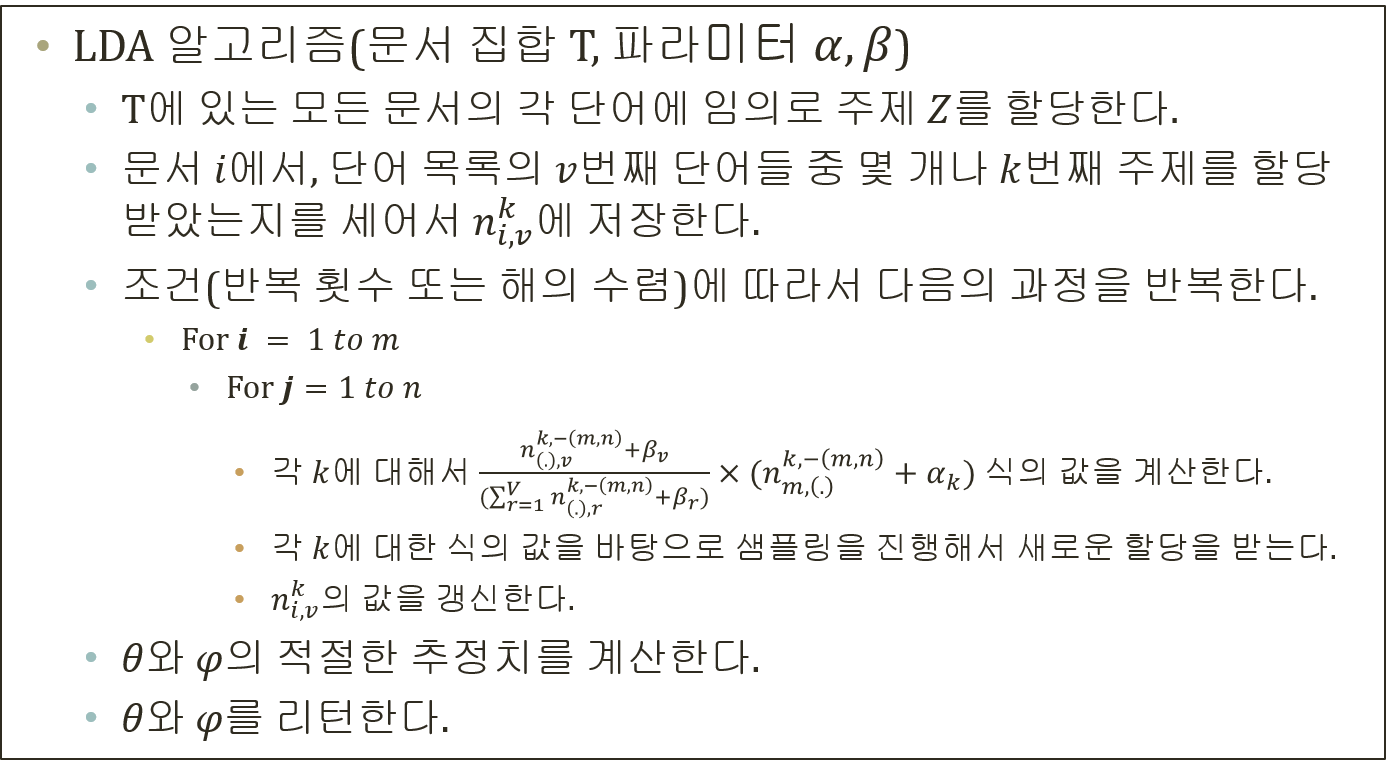
\includegraphics[scale=0.5]{fig10_26.png} 
\caption{전체 잠재 디리클레 할당 알고리즘 과정}
\label{fig:10-24}
\end{figure}
      
\end{document}